\documentclass[a4paper,12pt, notitlepage]{report}
\usepackage[T1]{fontenc}
\usepackage[utf8x]{inputenc}
\usepackage[english, frenchb, francais]{babel}
\usepackage{lmodern}
\usepackage{listings}
\usepackage{color}
\usepackage[margin=2.5cm, headheight=110pt]{geometry}
\usepackage{graphicx}
\usepackage{hyperref}
\usepackage{glossaries}
\usepackage{titlesec, blindtext, color}
\usepackage{fancyhdr}
\usepackage{datetime}
 
\definecolor{codegreen}{rgb}{0,0.6,0}
\definecolor{codegray}{rgb}{0.5,0.5,0.5}
\definecolor{codepurple}{rgb}{0.58,0,0.82}
\definecolor{backcolour}{rgb}{0.95,0.95,0.92}

\fancyhf{}
\pagestyle{fancy}
\fancyfoot[C]{\thepage}
\fancyhead[L]{Rapport de projet - Ecmchess}
\fancyhead[R]{\rightmark}

\lstdefinestyle{default}{
    backgroundcolor=\color{backcolour},   
    commentstyle=\color{codegreen},
    keywordstyle=\color{magenta},
    numberstyle=\tiny\color{codegray},
    stringstyle=\color{codepurple},
    basicstyle=\footnotesize,
    breakatwhitespace=false,         
    breaklines=true,                 
    captionpos=b,                    
    keepspaces=true,                 
    numbers=left,                    
    numbersep=5pt,                  
    showspaces=false,                
    showstringspaces=false,
    showtabs=false,                  
    tabsize=2
}

\lstset{language=php}  
\lstset{style=default}
\lstset{basicstyle=\footnotesize\ttfamily,breaklines=true}


\newglossaryentry{ORM}
{
  name=ORM,
  description={Object Relationnel Mapping. Technique de programmation faisant le lien entre le monde de la base de données et le monde de la programmation objet. Elle permet de transformer une table en un objet facilement manipulable via ses attributs}
}

\newglossaryentry{WYSIWYG}
{
  name=WYSIWYG,
  description={What You See Is What You Get : 
Le Wisiwig est une interface utilisateur qui permet de composer visuellement le résultat voulu, typiquement pour un logiciel de mise en page, un traiement de texte ou d’image. C'est une interface « intuitive » : l’utilisateur voit directement à l’écran à quoi ressemblera le résultat final
}
}

\newglossaryentry{bundle}
{
  name=Bundle Symfony,
  description={La traduction la plus proche d’un Bundle Synfony est le “module”, un bundle Symfony est un package regroupant une ou plusieurs fonctionnalités pouvant être ajouté à un site web Symfony pour faciliter sa création et/ou son  utilisation}
}

\newglossaryentry{service-container}
{
  name=Service Container,
  description={Ensemble de services, c'est-à-dire des classes PHP directement chargées et instanciées une seule fois au démarage du kernel (noyau) de Symfony. }
}

\newglossaryentry{entity-manager}
{
  name=Entity Manager,
  description={Classe permettant d'interfacer le monde de Doctrine et des classes implémentées par le développeur (Entité). En somme, il permet de gérer une entité depuis le code en appelant des méthodes raisonnant sur le modèle Objet}
}

\newglossaryentry{repository}
{
  name=Repository,
  description={Classe PHP implémentée par Symfony2 dépendant d'une entité permettant de définir
des requêtes DQL agissant sur son entité.}
}

\newglossaryentry{service}
{
  name=Service,
  description={Classe PHP instanciée une seule fois consistant en une fonctionnalité bien définie et pouvant être utilisée de n'importe où dans l'architecture mise en place par symfony (Injection de Dépendances)}
}

\makeglossaries

\definecolor{darkgrey}{RGB}{49,51,53}  
\definecolor{lightgray}{gray}{0.7}


\pagenumbering{Roman} 

\definecolor{gray75}{gray}{0.75}
\newcommand{\hsp}{\hspace{20pt}}
\titleformat{\chapter}[hang]{\Huge\bfseries}{\thechapter\hsp}{0pt}{\Huge\bfseries}


\title{Refonte du site web du club d'échec de Montpellier}
\author{Maxime Bertrand, Benjamin Hoquy, Sébastien Lacombe, Jason Thibur}



\begin{document}
\renewcommand{\contentsname}{Sommaire}
\renewcommand{\chaptername}{}
\renewcommand{\glossaryname}{Glossaire}
\pagestyle{empty}


\newdate{date}{23}{02}{2015}

\newcommand*{\plogo}{\fbox{$\mathcal{PL}$}} % Generic publisher logo

\newcommand{\titleGP}{\begingroup % Create the command for including the title page in the document
\centering % Center all text
\vspace*{\baselineskip} % White space at the top of the page

\rule{\textwidth}{1.6pt}\vspace*{-\baselineskip}\vspace*{2pt} % Thick horizontal line
\rule{\textwidth}{0.4pt}\\[\baselineskip] % Thin horizontal line

{\LARGE RAPPORT DE PROJET } \\[0.2\baselineskip] % Title

\rule{\textwidth}{0.4pt}\vspace*{-\baselineskip}\vspace{3.2pt} % Thin horizontal line
\rule{\textwidth}{1.6pt}\\[\baselineskip] % Thick horizontal line

\scshape % Small caps
Refonte du site web du club d'échecs de Montpellier \\ % Tagline(s) or further description
le \displaydate{date}, à Montpellier \\[\baselineskip] % Location and year


\includegraphics{images/ecmchess.png}
\vspace*{2\baselineskip} % Whitespace between location/year and editors

Réalisé par \\[\baselineskip]
{\Large Maxime BERTRAND \\ Benjamin HOQUY \\ Sébastien LACOMBE \\ Jason THIBUR \\[\baselineskip]} % Editor list
{\itshape IUT de Montpellier \\ pour l'obtention de la LP API-DAE \\[\baselineskip]} % Editor affiliation
{\large sous la direction de Xavier PALLEJA}

\vfill % Whitespace between editor names and publisher logo


\includegraphics[scale=0.4]{images/logoiut.jpg}

\includegraphics[scale=0.5]{images/um.png}

{\scshape Année universitaire 2014-2015} \\[0.3\baselineskip] % Year published
{\large }\par % Publisher

\endgroup}

\titleGP

\setcounter{page}{0}
\tableofcontents
\printglossaries

\pagestyle{fancy}
% REMERCIEMENTS %
\chapter*{Remerciements}
Nous aimerions remercier notre tuteur Xavier Palleja pour nous avoir guidé le long du projet tout en jouant le rôle du client exigeant et indécis.

Nous remercions aussi Mme Gelsomino pour son aide à la rédaction de ce rapport ainsi que M. Gautheret qui nous a initié à Symfony2.

% INTRODUCTION %
\chapter*{Introduction}
De nos jours, un site qui n’évolue pas n’attire pas les visiteurs. et lasse les coutumiers. Afin de garder un attrait, un site doit se renouveler de temps en temps. De plus, selon l’interface et les technologies utilisées la  gestion de son site peut rapidement devenir complexe et fastidieuse.

C’est dans ce contexte que le club d’échecs montpelliérain Echecs Club Montpellier souhaite faire une refonte de son site internet afin de lui donner un aspect plus jeune, ajouter une web-boutique et surtout faciliter la gestion de ses publications.

En effet, le site actuel ne permet qu’une gestion minimale et fastidieuse des articles. Avoir un back-office clair afin de gérer ses publications ainsi que les commentaires peut rendre cette tâche bien plus agréable et intuitive.

C’est autour de cette problématique que le club d’échecs nous a contacté pour développer une refonte de leur site internet plus simple d’utilisation et intégrant une boutique, en utilisant la technologie Symfony2.

Après avoir définis le cadre du projet et les besoins généraux de celui-ci dans l’analyse, nous détaillerons l’ensemble des fonctionnalités, l’architecture développées pour arriver au résultat final dans le rapport technique. Enfin nous reviendrons dans le rapport d’activité sur les méthodes ainsi que les différents outils de travail utilisés pour réaliser ce projet.

\newpage

\pagenumbering{arabic}







% ANALYSE %
\part{Analyse} 

\chapter{Analyse du contexte}
Le site du club d’échec de Montpellier a été développé avec Joomla pour une mise en place facile et rapide.
Jusqu’à lors le site ne permettait qu’à des administrateurs de gérer le contenu du site.

Le club désire donc que les membres inscrits aient la possibilité de proposer leurs propres articles et qu’une administration puisse vérifier la pertinence de ces derniers.

L’administration pourra quant à elle, revoir l’architecture du site (pages, menus et sous-menus) à tout moment et ainsi s’assurer de la bonne lisibilité des informations partagées. 

Le club possède une boutique physique interne et souhaiterait l’étendre sur son site web afin d’améliorer sa visibilité et son accessibilité. Pour cela, dans un premier temps il faudra mettre en place une vitrine informative des produits, et, le cas échéant donner la possibilité aux membres et aux visiteurs du site de passer leur commandes en ligne.

\chapter{Analyse des besoins fonctionnels}
Le nouveau site développé devra inclure:
\begin{itemize}
\item{une vitrine présentant le club (informations essentielles, contact, sponsors)}
\item{une boutique en ligne}
\item{une partie administration ou back office}
\item{une partie publication d’articles concernant le club}
\end{itemize}

L’utilisateur enregistré pourra:

\begin{itemize}
\item{consulter les nouveautés publiées par les autres utilisateurs enregistrés}
\item{publier des articles dans les sections autorisées}
\item{acheter différents produits vendus dans la boutique}
\end{itemize}

L’administrateur pourra:
\begin{itemize}
\item{modérer les articles publiés par les utilisateurs enregistrés}
\item{modifier les informations essentielles statiques de la vitrine (contact, cours, organigramme, sponsors, etc.)}
\item{gérer la boutique}
\item{gérer l’architecture du site (navigation)}
\end{itemize}


\chapter{Analyse des besoins non fonctionnels}
\section{Contraintes techniques}
Le site devra être développé avec le framework Symfony 2.
\section{Contraintes ergonomiques}
La charte graphique du site devra concorder avec les couleurs du club et de la commune(bleu).

\chapter{Scénarios des cas d'utilisations}
\begin{figure} 
    \caption{Diagramme des cas d'utilisation}  
    \label{use-case}
    \centering
    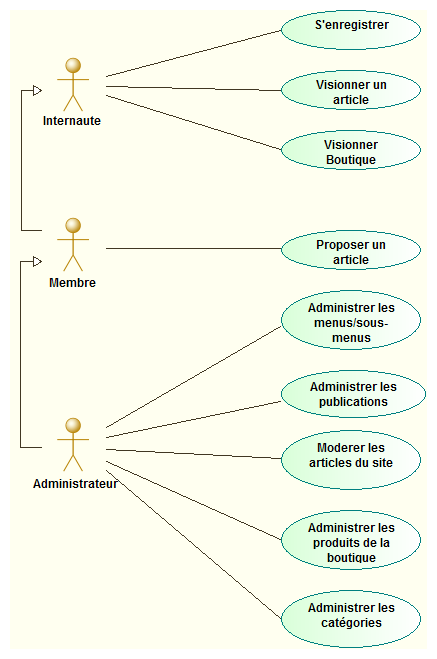
\includegraphics[scale=0.8]{images/diagUseCase.png}
\end{figure}
\section{Scénarios utilisateur non connecté}
\subsection{S'inscrire sur le site}
\begin{enumerate}
    \item L'internaute clique sur le bouton « Inscription » 
    \item Le système affiche le formulaire d'inscription et demande à l'internaute de le remplir 
    \item L'internaute rempli le formulaire et appuie sur le bouton « Valider » 
    \item Le système envoie un mail de validation d'inscription à l'internaute contenant la lien pour terminer l'inscription. 
    \item L'internaute clique sur le lien de validation et termine son inscription. 
    \item Le système active le compte et affiche à l'internaute que l'inscription s'est bien finalisée 
\end{enumerate}
\subsection{Se connecter}
\begin{enumerate}
    \item L'internaute clique sur le bouton « S’authentifier » 
    \item Le système affiche le formulaire de connexion 
    \item L'internaute rempli les champs du formulaire de connexion et appuie sur le bouton « Connexion » 
    \item Le système vérifie la validité des identifiants saisis précédemment 
    \item L'internaute est redirigé sur la « page d'accueil » avec un message de bienvenue et un onglet « mon compte » 
\end{enumerate}
\section{Scénarios utilisateur}
\subsection{Publier un article}
\begin{enumerate}
    \item L’utilisateur clique sur “Proposer un article” 
    \item Le système affiche un formulaire contenant les informations essentielles d’un menu
    \item L’utilisateur renseigne les champs du formulaire et le valide
    \item Le sytème affiche un message de validation de l’article, l’article ne sera affiché que si un administrateur valide l’article
\end{enumerate}
\subsection{Modifier un article}
\begin{enumerate}
    \item L’utilisateur clique sur “Mes article” 
    \item L’utilisateur sélectionne l’article a modifier, le motif de refus est afficher 
    \item Le système affiche un formulaire contenant les informations essentielles
    \item L’utilisateur modifier les champs du formulaire et le valide
    \item Le sytème affiche un message de validation de l’article, l’article ne sera affiché que si un administrateur valide l’article
\end{enumerate}
\section{Scénarios administrateur}
\subsection{Ajouter un menu/sous-menu}
Ajout d'un menu
\begin{enumerate}
    \item L’administrateur va dans l’interface d’administration 
    \item L’administrateur clique sur le bouton “Ajouter un menu”
    \item Le système affiche un formulaire contenant les informations essentielles d’un menu
    \item L’administrateur renseigne les champs du formulaire et le valide
    \item Le sytème affiche un message de validation de création du menu
\end{enumerate}

Ajout d'un sous-menu
\begin{enumerate}
    \item L’administrateur va dans l’interface d’administration 
    \item L’administrateur clique sur le bouton “Ajouter un sous-menu”
    \item Le système affiche un formulaire contenant les informations essentielles d’un sous-menu
	    ainsi qu’une liste déroulante avec les diffèrent menu. 
    \item L’administrateur renseigne les champs du formulaire et le valide
    \item Le sytème affiche un message de validation de création du menu
\end{enumerate}
\subsection{Accéder à l'interface d'administration}
\begin{enumerate}
    \item{L'administrateur clique sur l'onglet du menu « Administration » (disponible que pour l'administrateur)}
    \item{Le système affiche la page d'administration contenant les liens pour administrer les différentes partie du site}
    \item{Le système affiche les différentes parties que l'administrateur peut modifier sous forme de liens}
\end{enumerate}

\subsection{Ajouter un sponsor}
\begin{enumerate}
    \item{L'administrateur clique sur le lien modifier les sponsors.}
    \item{Le système affiche la liste ordonnée des sponsors avec la possibilité de les modifier (ajout/suppression/modification)}
    \item{L'administrateur clique sur « ajouter ».}
    \item{Le système affiche un formulaire avec les informations du sponsor à renseigner (sous forme de formulaire : nom, lien hypertexte, ordre, image).}
    \item{L'administrateur renseigne les champs et valide l'ajout.}
    \item{Le système affiche un message de confirmation.}
\end{enumerate}
\subsection{Ajouter une publication}
\begin{enumerate}
    \item L’administrateur va dans l’interface d’administration 
    \item L’administrateur clique le bouton “Publication”
    \item Le système affiche les publications présents sur le site ainsi que l’option d’ajout d’une publication
    \item L’administrateur clique sur le bouton “Ajouter une publication”
    \item Le système affiche un formulaire contenant les informations essentielles d’une publication
    \item L’administrateur renseigne les champs du formulaire et le valide
    \item Le sytème affiche un message de validation de création de l’article dans le menu
\end{enumerate}
\subsection{Refuser un article}
\begin{enumerate}
    \item L’administrateur va dans l’interface d’administration
    \item L’adminstrateur clique sur “Article”
    \item L’administrateur  clique sur l’article a refuser 
    \item L’administrateur selectionne et “refuser” et met un motif de refus puis valide le formulaire 
    \item Le sytème affiche un message de validation, l’article sera pas visible sur le site, l’utilisateur devra modifier sont article pour qu’il soit ressoumit a une validation par l’administrateur.
\end{enumerate}
\subsection{Valider un article}
\begin{enumerate}
    \item L’administrateur va dans l’interface d’administration
    \item L’adminstrateur clique sur “Article”
    \item L’administrateur  clique sur l’article a valider
    \item L’administrateur selectionne et “valider” et valide le formulaire 
    \item Le sytème affiche un message de validation, l’article sera visible sur le site
\end{enumerate}











% RAPPORT TECHNIQUE %
\part{Rapport technique}



\chapter{Conception}


\section{Présentation des choix technologiques}
\subsection{Langages de programmation}
\subsubsection{Langage principal}
PHP5 (utilisé par Symfony2)
\subsubsection{Langages de requêtes}
\emph{MySQL, DQL (Doctrine Query Language)} : langage de requête utilisé par Doctrine dérivant du SQL. La différence majeure est que le DQL exécute des requêtes sur des entités Doctrine au lieu de les faire sur des tables SQL.
\subsection{Langages de structuration des données}
\begin{itemize}
    \item \emph Twig : moteur de template présent par défaut dans Symfony2
    \item \emph HTML5 
    \item \emph CSS3
\end{itemize}

\subsection{Langages de configuration}
\begin{itemize}
    \item \emph YML : langage de configuration utilisé par Symfony2 décrivant plusieurs objets (attribut, valeur) servant à la configuration de Symfony et/ou de ses modules.
    \item \emph XML 
\end{itemize}
\section{Framework et outils intégrés}
\begin{itemize}
    \item \emph Symfony: Framework français écrit en PHP5, et conçu pour développer des applications en 3 couches, selon le modèle MVC (voir figure \ref{request-flow}), permettant de produire du code propre et organisé.
    \item \emph Doctrine : \gls{ORM} intégré par défaut dans le moteur de Symfony2. Il sert de couche de relation entre la base de données et les entités et permet d’interfacer les actions pouvant être appelées sur les entités en langage objet
\end{itemize}

\begin{figure} 
    \caption{Fonctionnement de Symfony 2}  
    \label{request-flow}
    \centering
    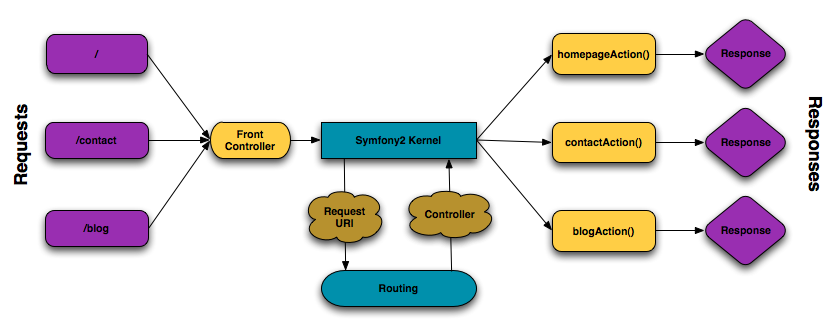
\includegraphics[scale=0.5]{images/request-flow.png}
\end{figure}

\section{Description des fonctionnalités}
\subsection{Création d'une publication}
Une distinction a été faite entre les publications et les articles.Un article est rédigé par un utilisateur membre. Une publication, quant à elle, ne peut être créée que par l'administrateur du site. De ce fait, la création se fait sur l'interface d'administration et utilise, par conséquent, le module Sonata Admin Bundle.
\subsubsection{Sonata Admin Bundle}
Sonata Admin Bundle est un module pour Symfony permettant d'administrer des entités Doctrine. Il est nécessaire d'implémenter une classe XxxAdmin héritant de Sonata/AdminBundle/Admin/Admin contenant des méthodes permettant de mapper les attributs de l'entité. Ce mapping est configuré dans le fichier services.yml.
\lstinputlisting[firstline=18, lastline=28, language=php]{../src/ECM/Bundle/ArticleBundle/Resources/config/services.yml}
La classe précisée dans l'attribut \verb?class? (ECM/Bundle/ArticleBundle/Admin/ArticleAdmin) sera utilisée par Sonata pour mapper les attributs de l'entité passée en argument dans l'attribut \verb?arguments? (ECM/Bundle/ArticleBundle/Entity/Article).
\lstinputlisting[firstline=47, lastline=55, language=php]{../src/ECM/Bundle/ArticleBundle/Admin/ArticleAdmin.php}
Une fois la relation indiquée, il reste à signaler à Sonata les éléments à afficher sur son interface d'administration. La méthode configureFormFields indique à Sonata quels champs de l'entité Article seront affichés lors de la modification d'un article.
\subsubsection{CKEditor}
CKEditor est un éditeur de texte open source de type \gls{WYSIWYG} pouvant servir à la création de contenu de pages web.
Toute rédaction de texte liée à la publication d’articles est faite à l’aide de CKEditor.
\lstinputlisting[firstline=13, lastline=30, language=php]{../src/ECM/Bundle/ArticleBundle/Form/ArticleType.php}
Lors de la création du formulaire (buildForm()), la classe “ ckeditor ” est passée en paramètre au champ “corps” qui est de type texte.
Durant la génération du formulaire, la zone de texte du champ “corps” sera replacé par l’interface d’édition de ckeditor (voir figure \ref{ckeditor})
\begin{figure} 
    \caption{Zone d'édition CKEditor}  
    \label{ckeditor}
    \centering
    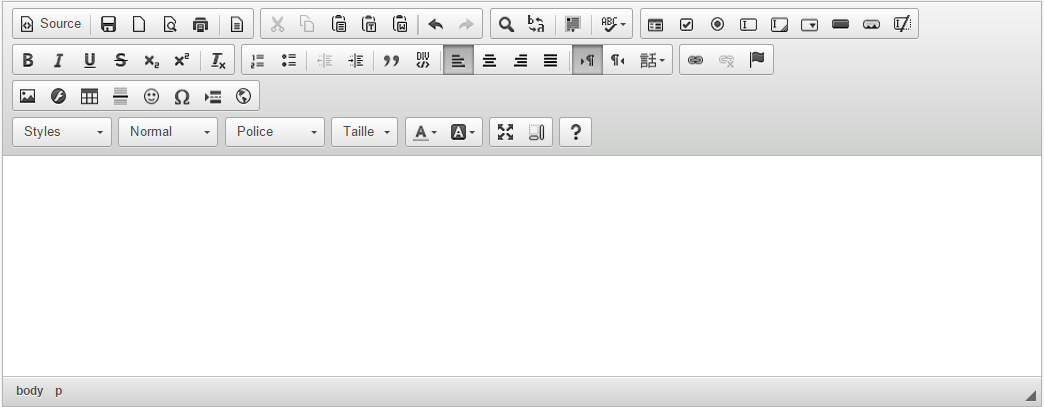
\includegraphics[scale=0.5]{images/ckeditor.png}
\end{figure}
\subsection{Administration générale}
\subsection{Gestion des articles}
\begin{figure} 
    \caption{Diagramme d'État-transition d'un article}  
    \label{e-t-articles}
    \centering
    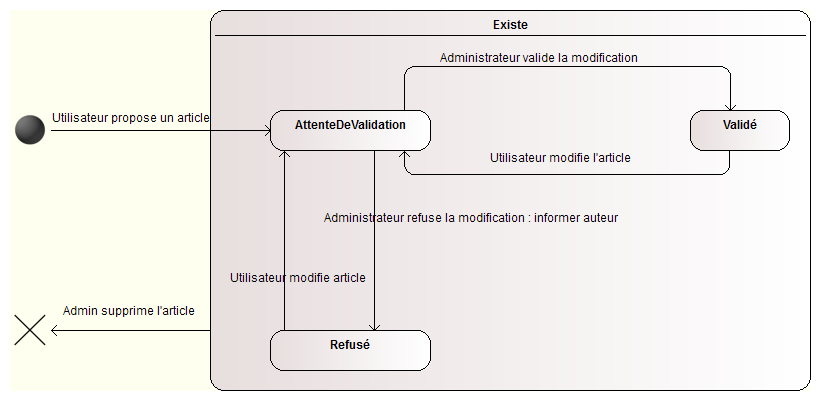
\includegraphics[scale=0.37]{images/DiagEtatTransitionEtatArticle.png}
\end{figure}
\subsubsection{Proposition d'un article}
\begin{figure}
    \caption{Proposer un article}  
    \label{proposer-article}
    \centering
    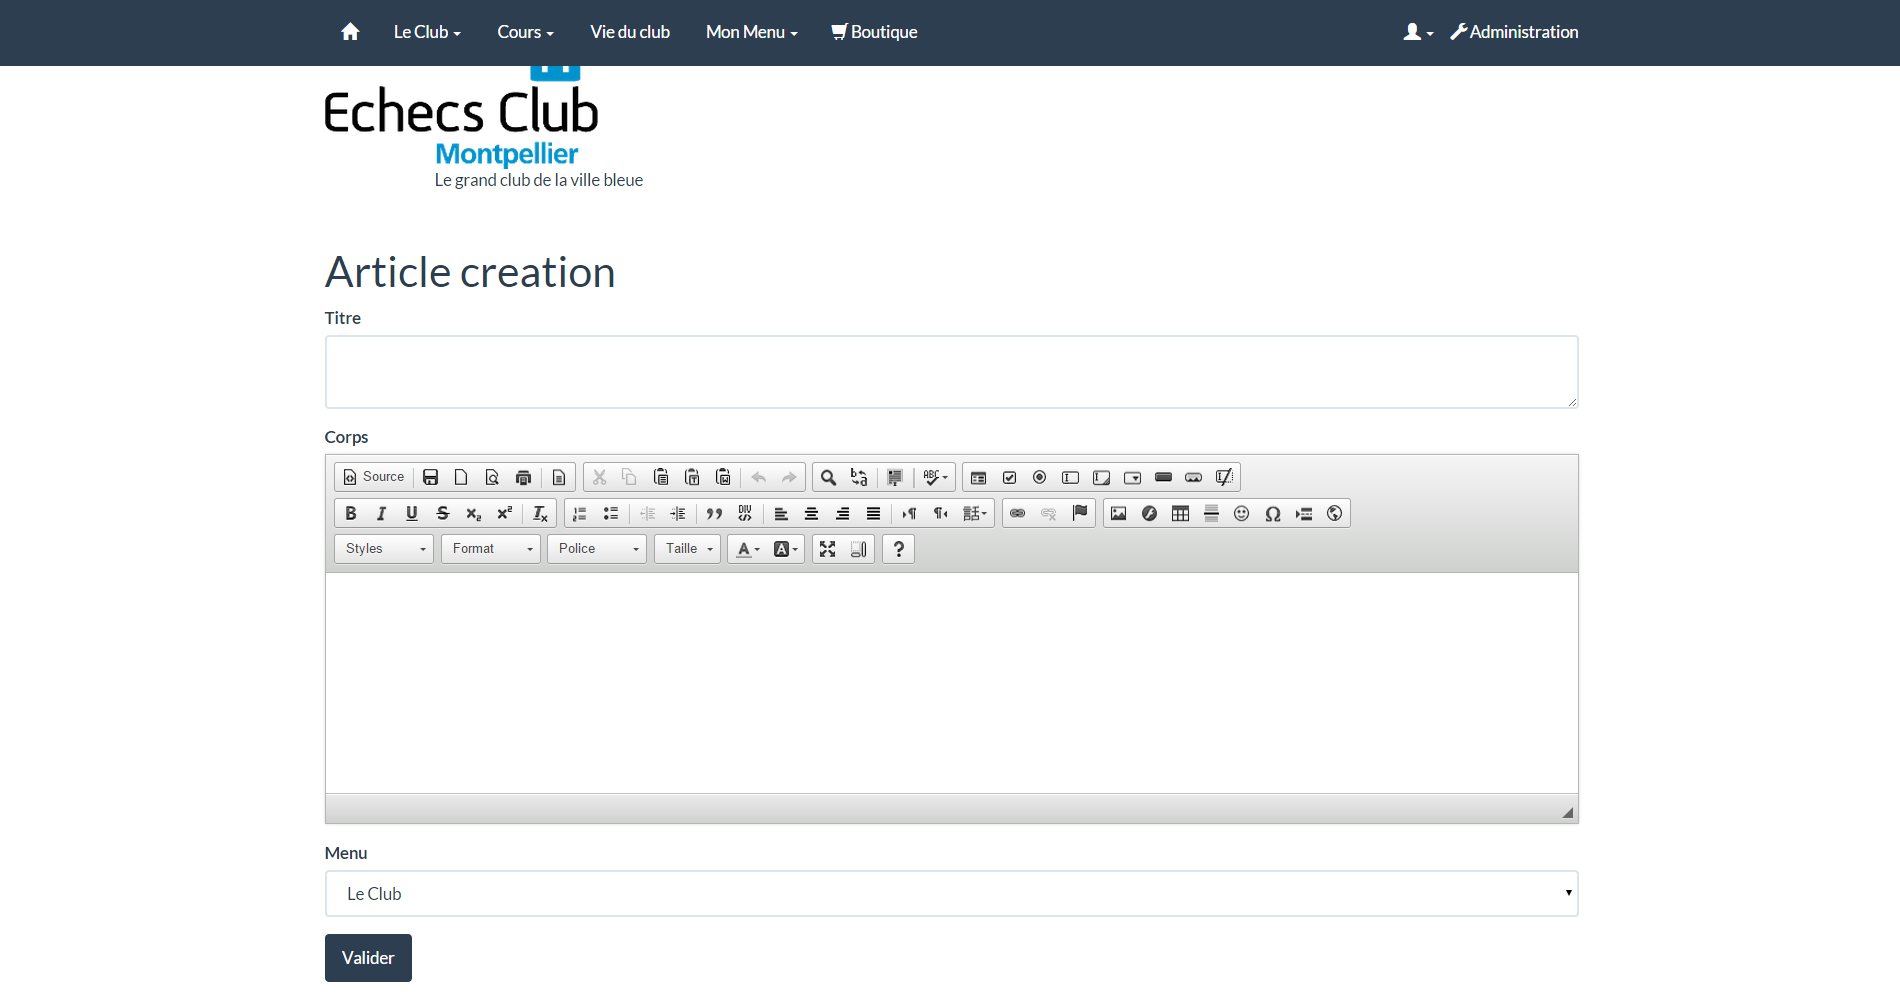
\includegraphics[scale=0.3]{images/proposer-article.png}
\end{figure}
Lorsque l’utilisateur demande à poster un article(voir figure \ref{proposer-article}), une entité Article est automatiquement créée par le contrôleur d’articles c’est à partir de cette entité que le contrôleur génère une vue avec les champs adaptés pour ensuite l’envoyer à l’utilisateur.

\lstinputlisting[firstline=47, lastline=70, language=php]{../src/ECM/Bundle/ArticleBundle/Controller/ArticleController.php}
Une fois les champs remplis, l’utilisateur appuie sur le bouton de soumission. Le contrôleur d’article demande au \gls{service-container} de lui donner l’ \gls{entity-manager} qui s’occupe alors de stocker l’entité dans la base de données (persist(entity)), puis qui valide les changements effectués dans la base (flush()).

L’article est alors créé, en attente de validation par l’administrateur. Il sera donc caché jusqu’à sa validation, l’auteur pourra tout de même vérifier l’état de son article ou le modifier à sa convence.
\begin{figure} 
    \caption{Diagramme de Séquence - Proposer un article}  
    \label{seq-proposer-article}
    \centering
    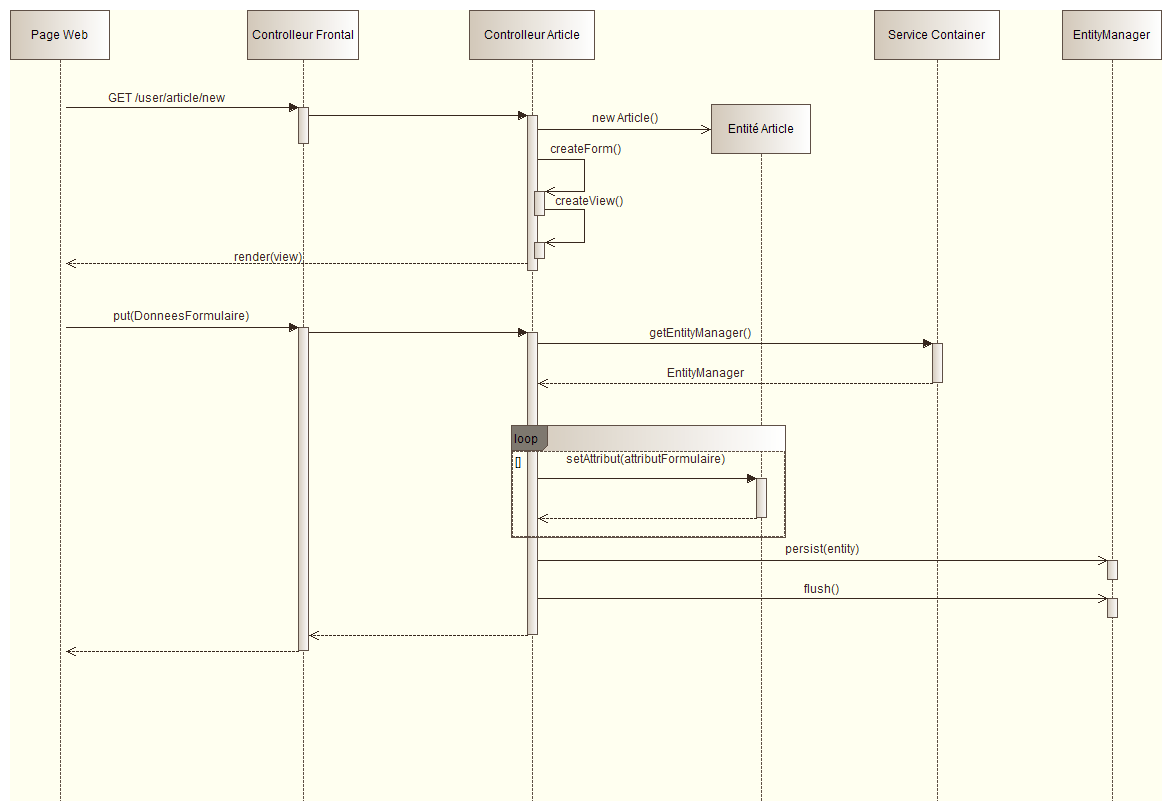
\includegraphics[scale=0.37]{images/DiaSequenceProposerArticle.png}
\end{figure}
\subsubsection{Modération d'un article}
Lorsque l’administrateur demande à afficher la liste des articles pour les administrer, le contrôleur article demande au \gls{service-container} le \gls{repository} de l'article en charge de récupérer les données de la base. Le contrôleur demande alors de récupérer tout les articles (findAll()), la liste des articles est alors renvoyée directement à la vue qui récupère les attributs nécessaires à la liste de chacun des articles. Ces étapes sont implicitement gérées par Sonata Admin \gls{bundle}
\begin{figure} 
    \caption{Liste des articles sur l'interface d'administration}  
    \label{liste-article}
    \centering
    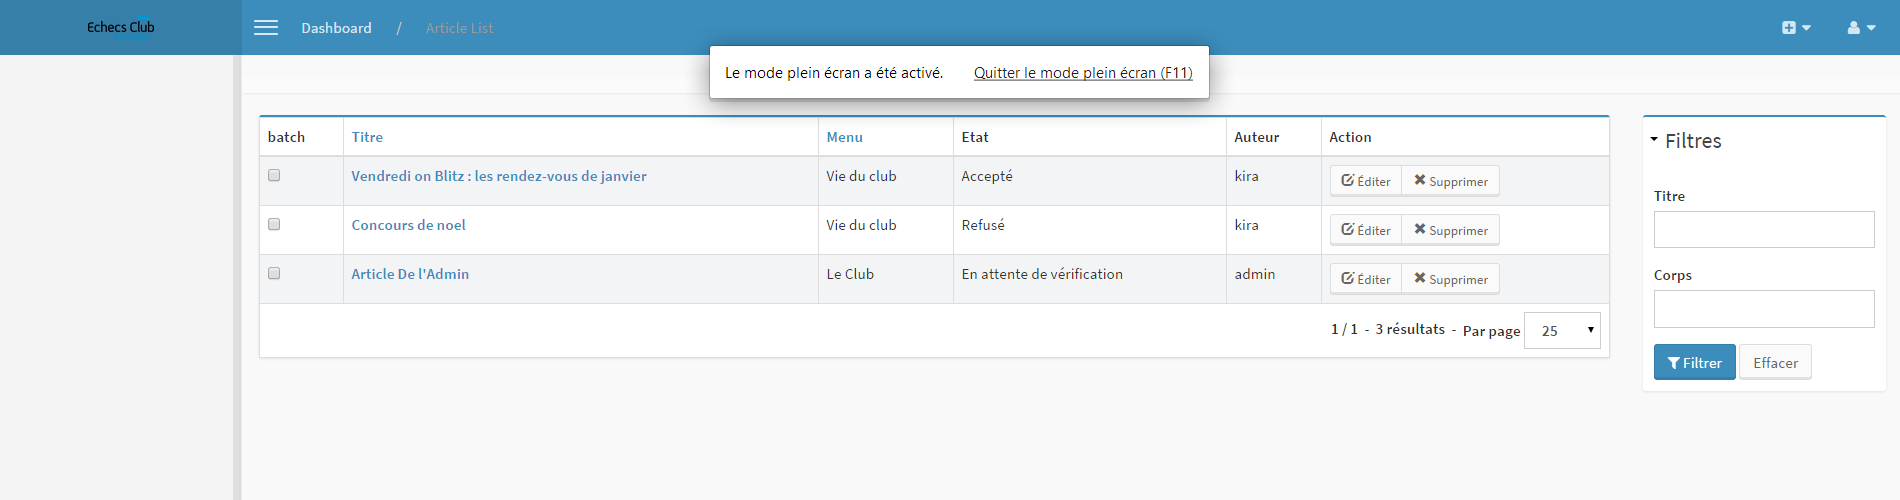
\includegraphics[scale=0.3]{images/liste-article.png}
\end{figure}

Une fois que l’administrateur a choisi quel article modérer, il le sélectionne. De la même manière, le contrôleur demande au \gls{repository} de l'article de lui trouver l’article en question à partir de son ID (findByID(idArticle)), de la même manière l’article est retrouné à la vue qui génère le formulaire en fonction des attributs à afficher (titre, auteur, corp, menu d’appartenance) (voir figure \ref{modif-article}).

\begin{figure} 
    \caption{Modification d'un article sur l'interface d'administration}  
    \label{modif-article}
    \centering
    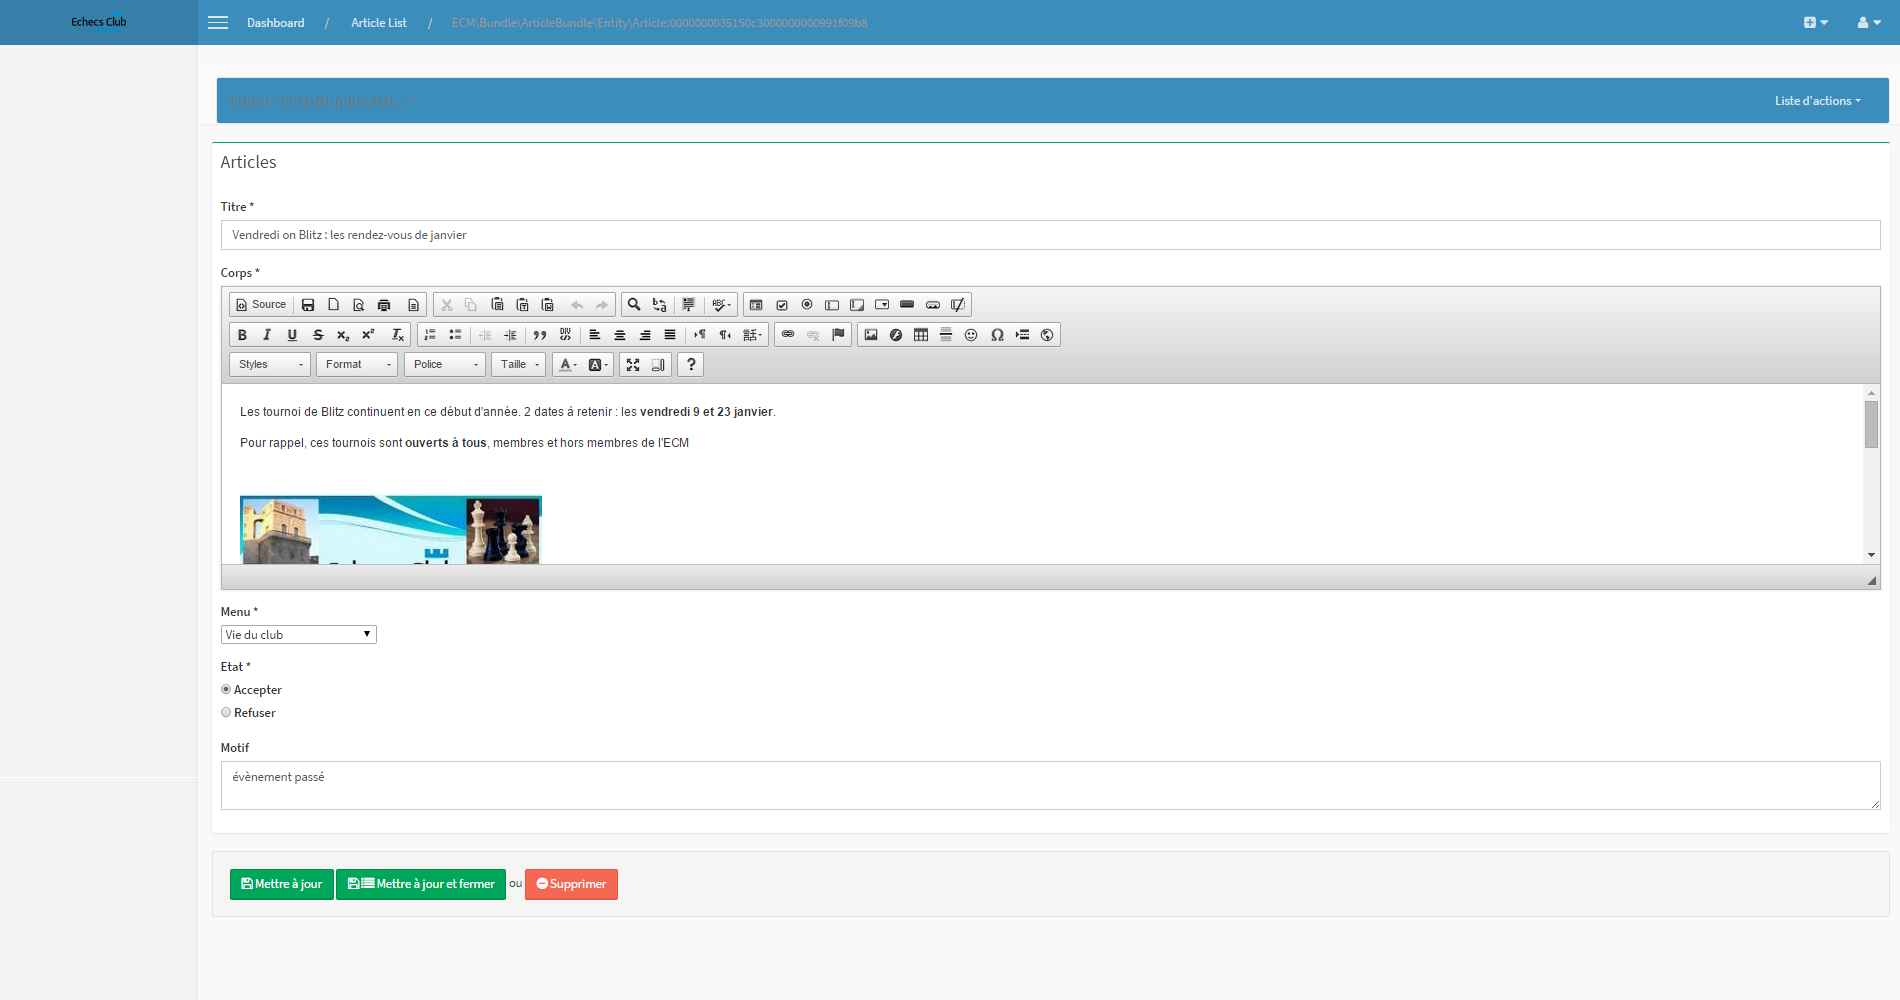
\includegraphics[scale=0.3]{images/modif-article.png}
\end{figure}

Après lecture l’administrateur choisi soit de le valider, soit de le refuser via les boutons radios de la page.
Pour l’enregistrement des changements, le contrôleur fait appel à l’EntityManager à qui il demande de valider les changements fait en effectuant un flush()(voir figure \ref{admin-article}).

\begin{figure} 
    \caption{Diagramme de Séquence - Administration d'un article}  
    \label{admin-article}
    \centering
    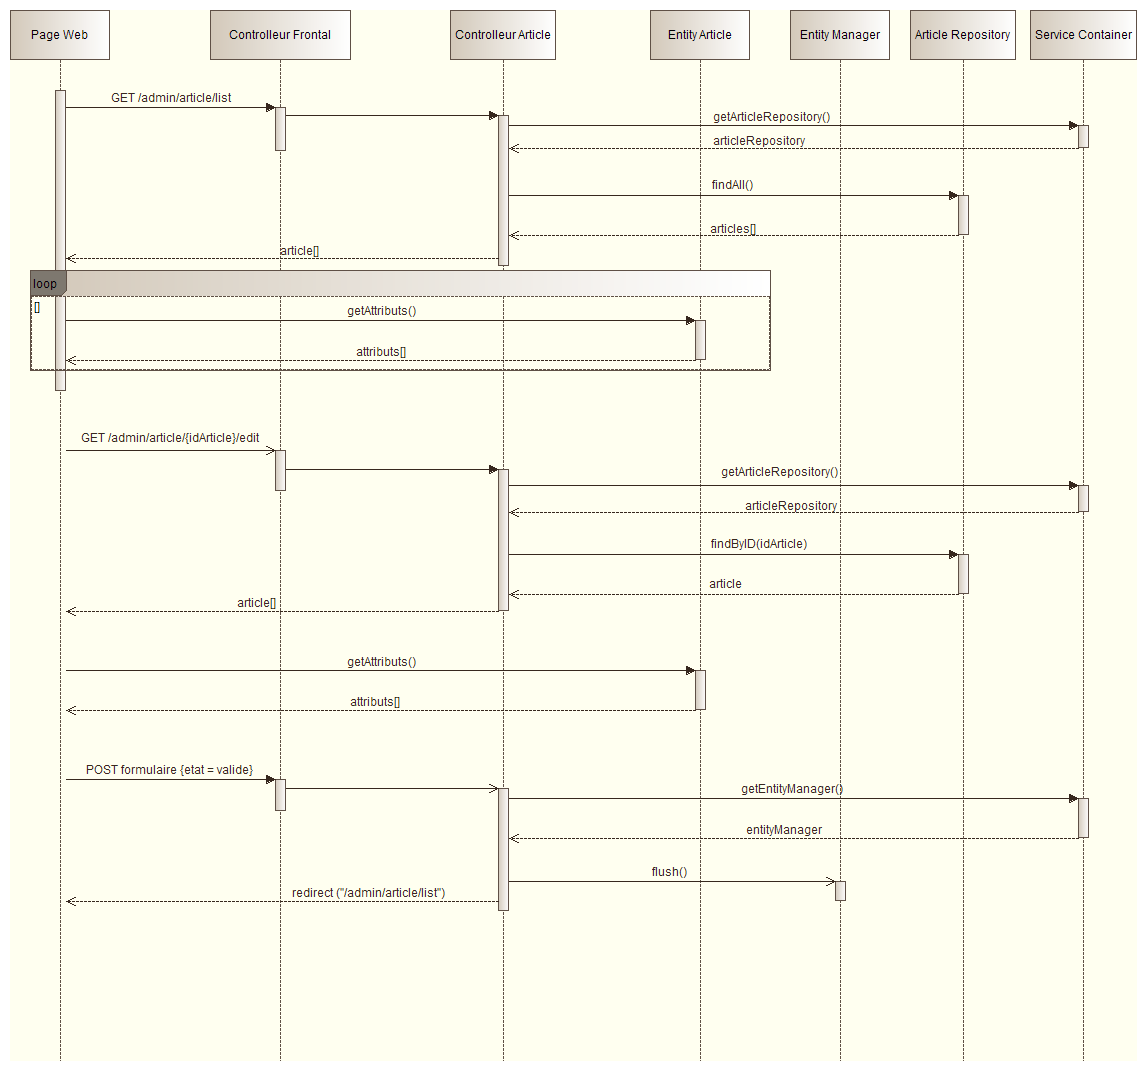
\includegraphics[scale=0.38]{images/DiagSequenceAdministrationArticle.png}
\end{figure}

\subsection{Gestion des menus/sous-menus}
\subsubsection{Menus statiques}
KNP Menu Bundle est utilisé pour la création et l’affichage des menus.
Le bouton “Administration” va servir d’exemple pour essayer de comprendre le fonctionnement des menus statiques(voir figure \ref{btn-admin}).
\begin{figure} 
    \caption{Menu Administration}  
    \label{btn-admin}
    \centering
    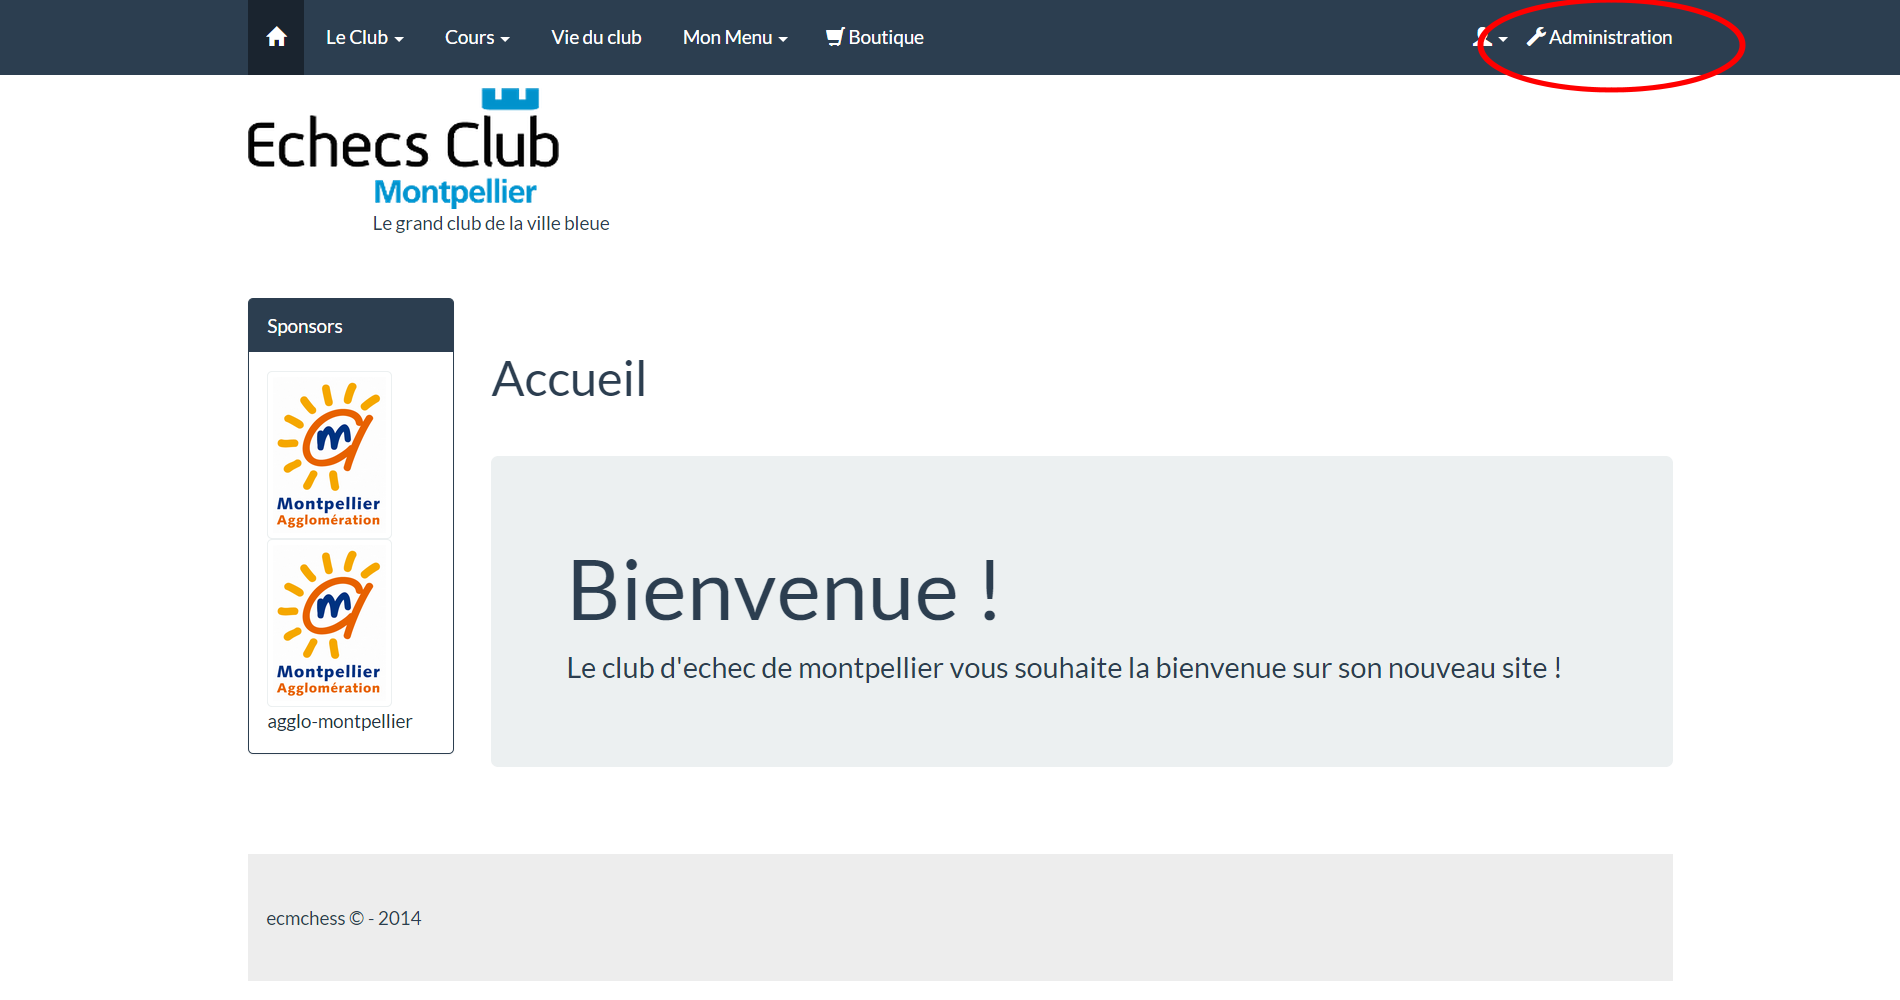
\includegraphics[scale=0.3]{images/btn-admin.png}
\end{figure}
\lstinputlisting[language=html]{../app/Resources/views/menu.html.twig}
Toujours pour suivre l’exemple avec le menu “Administration”, la vue vérifie si l’utilisateur en cours est connecté en tant que “ROLE\_ADMIN” grâce au test is\_granted.
S’il est connecté en tant qu'admin, la vue appelle le \gls{service} “admin” qui se charge d'afficher le menu administrateur.
\lstinputlisting[firstline=27, lastline=34, language=html]{../src/ECM/Bundle/HomeBundle/Resources/config/services.yml}
Le \gls{service} ecm\_home.menu.admin sert à appeler la méthode “createAdminMenu()” de la classe MenuBuilder. Il est utile de préciser que la requête (@request) est injectée dans le menuBuilder.

Cette méthode de la classe menuBuilder sert à la création du menu “Administration”
Le menu retourné (menu) est contruit à partir de KNP/Menu/FactoryInterface.
La fonction setChildrenAttribute sert a appliquer la classe css ‘nav navbar-nav’ au menu,
la classe ‘nav navbar-nav’ est une classe Bootstrap, elle sert à la mise en forme du menu.
Ensuite la fonction ‘addChild’ ajoute un enfant au menu en lui donnant en paramètre le libellé du menu (‘Administration’) et la route qui sera appelée lors du clique sur le menu (\verb?route => sonata_admin_dashboard?) qui provient du fichier config.yml.
La fonction “setAttribute” ajoute un attribut de type glyphicon de valeur “wrench” au menu.
\lstinputlisting[firstline=25, lastline=36, language=php]{../src/ECM/Bundle/HomeBundle/Menu/MenuBuilder.php}
Enfin, la méthode renvoie le menu à la vue qui se charge de l’afficher.

\subsubsection{Menus Dynamiques}
Il est possible de créer des menus personnalisés via l'interface d'administration. Ces menus peuvent également contenir des sous-menus.
Pour gérer ce type d'architecture, un héritage entre menu et sous-menu est nécessaire. 

Le processus d'affichage avec KNPMenuBundle ainsi que le \gls{service} utilisé pour générer le menu sont les mêmes que pour les menus statiques.
\subsubsection{Héritage}
L'héritage se configure dans les classes des entités Doctrine (Menu et SubMenu en l'occurrence).
\lstinputlisting[firstline=9, lastline=19, language=php]{../src/ECM/Bundle/ModuleBundle/Entity/Menu.php}
\lstinputlisting[firstline=7, lastline=14, language=php]{../src/ECM/Bundle/ModuleBundle/Entity/SubMenu.php}
\verb?Inheritance Type? sert à déterminer comment Doctrine converti cet héritage en tables SQL (soit \verb?JOINED?, ou \verb?SINGLE_TABLE?). Ici, \verb?JOINED? fait en sorte que deux tables soient crées (Menu et SubMenu). Menu contient un attribut discriminant (spécifié dans \verb?Discriminator Column?) faisant la différence entre un Menu et un SubMenu. Lorsque ce discrimant vaut "menu", doctrine sait que c'est un menu. Au contraire lorsqu'il vaut "submenu", il sait que c'est un sous-menu et référence directement ce sous-menu dans l'autre table SQL SubMenu contenant tous les attributs spécifiés dans SubMenu et pas dans Menu.
\subsubsection{Conteneur de Menus}
Un \gls{service} jouant le rôle d'un \gls{repository} permet d'accéder aux menus contenus dans la base de données depuis le MenuBuilder de KNP. 

Deux méthodes sont implémentées :
\begin{itemize}
    \item getMenus permettant de récupérer tous les menus (et seulement les menus)
    \item getSubMenus permettant de récupérer tous les enfants d'un menu
\end{itemize}
\lstinputlisting[firstline=14, lastline=30, language=php]{../src/ECM/Bundle/HomeBundle/MenusContainer/MenusContainer.php}

La configuration de ce service se situe dans le fichier services.yml du bundle HomeBundle. Grâce à ce fichier, le \gls{service} est enregistré par le kernel de Symfony dans le \gls{service-container}.
\lstinputlisting[firstline=14, lastline=17, language=html]{../src/ECM/Bundle/HomeBundle/Resources/config/services.yml}


\subsubsection{Affichage des menus et sous-menus}

Pour afficher les menus et sous-menus, la fonction \verb?generateMenu()? parcourt le tableau de menus renvoyé par le conteneur de menus (\verb?getMenus()?).
Pour chaque menu, tous ses potentiels enfants sont récupérés et sont ajoutés en tant qu'enfant, via \verb?addChild()?, au menu parent.
\lstinputlisting[firstline=81, lastline=101, language=php]{../src/ECM/Bundle/HomeBundle/Menu/MenuBuilder.php}
\subsubsection{Slugify}
Slugify est un petit module permettant de créer des slugs (jetons fabriqués à la volée à partir de chaînes de caractères). En l'occurence, ce module est utilisé pour générer des chaînes de caractères compatibles aux URLs (pour les menus).

\subsection{Gestion des utilisateurs}
Cette partie a été développé à l'aide du bundle FOSUserBundle.
\subsubsection{FOSUserBundle}
FOSUser sert à la gestion des membres (inscription / connexion / déconnexion / changement de mot de passe )
\lstinputlisting[firstline=156, lastline=165, language=python]{../app/config/config.yml}
Un UserBundle a été développé pour gérer les utilisateurs. Ce \gls{bundle} étend de FOSUser, il hérite donc de toutes les méthodes et les fonctionnalités que propose FOSUserBundle. La mise en place de ce \gls{bundle} est simple: il suffit de spécifier la classe que l'on veut faire hériter de FOSUser UserBase.  
\subsection{Gestion des sponsors}
La gestion de l'administration des sponsors est la même que pour les autres fonctionnalités (mapping de l'entité et configuration des champs affichés dans une classe \verb?XxxAdmin?). Cependant, la gestion des sponsors nécessite un petit module permettant d'ordonner la position des sponsors.
\subsubsection{Pix Sortable Bundle}
Pix Sortable Bundle est un \gls{bundle} qui permet de trier et d'ordonner toute sorte entité.
Pix Sortable Bundle sert à l'ordonnancement des sponsors, c’est à dire qu’il est possible de modifier l’ordre d’affichage des sponsors. 
Une petite fonction intégrée à \verb?SponsorAdmin? permet d'interfacer ce module avec Sonata 


\chapter{Résultats et perspectives}
\section{Résultats}
\subsection{Vitrine}
Le site contient une vitrine servant à présenter le club aux futurs adhérents ou aux personnes recherchant des informations sur le club. Mais aussi aux adhérents qui veulent se tenir informés des différentes news et évènements.

L’administrateur peut ajouter, modifier ou supprimer des publications ce qui rend la vitrine parfaitement dynamique.
\subsection{Inscription d'un membre}
Les internautes désirant s’inscrire au site, peuvent le faire via un formulaire dédié. Les inscriptions doivent être validées par mail ce qui a pour but d'empêcher les robots de s'inscrire.

Une fois inscrit, un utilisateur peut modifier sont mot de passe via le formulaire adéquat.
\subsection{Gestion des articles/sponsors}
Le site permet à l’administrateur de gérer les sponsors. Il permet d’en créer, de les modifier, ou de les supprimer, mais aussi de trier l’ordre d’affichage, en fonction de leur importance, les sponsors affichés sur le site (amenant sur le site web du sponsor).

Le site  possède un système de publication et de modération des articles, un utilisateur inscrit peut proposer un article, via un formulaire correspondant.
Cet article une fois validé est soumis à la modération de l’admin. Si l’article et accepté, il sera affiché sur le site. Dans le cas contraire l’utilisateur est invité à modifier son article.

\subsection{Gestion des catégories/produits}
Le site contient la liste des produits vendus par le club en fonction de leur catégorie. 
Ces produits et ces catégories sont donc administrables, l’administrateur peut créer, modifier ou supprimer des catégories. Le site permet la création, la modification et la suppression des produits, les produits appartiennent à une catégorie.

\section{Perspectives}
\subsection{Boutique}
Dans une évolution future, il sera utile d’ajouter un panier et de finaliser la partie boutique du site web, pour que les utilisateurs puissent acheter les produits directement sur le site web.
\subsection{Gestion d'équipes}
Il serait aussi possible d’ajouter une partie "équipes", pour faciliter la gestion de ces dernières par les chefs d’équipe lors de l’organisation de tournois.
\subsection{Gestion des membres/inscription}
Il faudrait rajouter une gestion des membres ainsi qu’un système permettant seulement aux adhérents du club de s’inscrire au site, ou de poster des articles. Une réunion avec le client devrait se faire pour décider de la solution la plus adaptée.

% RAPPORT D'ACTIVITÉ %
\part{Rapport d'activité}
\subsubsection{Gestion des itérations}
Pour le démarrage du projet, nous avons fait une réunion avec notre tuteur, M. Palleja où nous avons discuté de ses attentes et du contenu global du projet. Nous avons fait un rapport préliminaire afin de bien vérifier la bonne compréhension du sujet que nous avons rendu la semaine suivante. Lors de la réunion qui suivi le rendu du rapport nous avons pu débattre des idée et proposition que nous avions à faire avant de nous lancer totalement dans le projet.

Par la suite, nous avons suivis une démarche agile en travaillant par itérations de deux semaines durant la période de cours, et en réduisant ce délais de moitié pour les dernières semaines consacrées au projet. Pour l’intégration nous avons utilisé le gestionnaire de version Git que nous avons intégré à nos Environnements de développement . Nous avons mis en place un Kanban via la site de Trello pour nous répartir les tâches lors des premières itérations.
 
\subsubsection{Difficultés rencontrées}
Mais, face aux difficultés techniques que nous avons rencontrées quant à l’utilisation de Sonata, nous nous sommes regroupés derrière un seul codeur pour comprendre le fonctionnement  de Sonata et le mettre en place…
Une fois ceci fait, nous avons réussi à nous diviser en deux équipes afin de terminer la mise en place de la gestion des articles et de la boutique.

\subsubsection{Conclusion}
En revenant sur notre progression, il aurait été préférable de ne pas utiliser Sonata Admin Bundle pour la gestion du site car, bien que ce module soit performant, l’équipe ne possédait pas les compétences nécessaires pour sa mise en place dans un délai acceptable. De plus, le module possédait énormément de fonctionnalités superflues pour notre projet. Une recherche plus approfondie d’un autre module, voire s’en passer aurait sûrement été préférable. D’un autre coté, d’un point de vue pédagogique l’installation de Sonata nous a permis de mieux comprendre le fonctionnement de Symfony2 et de l’installation de modules, l’installation de Sonata n’a pas été une totale perte de temps.


% MANUEL D'UTILISATION %
\part{Manuel d'utilisation}
\chapter{Accéder à l'interface d'administration}
Pour pouvoir accéder au back office il faut dans un premier temps, se connecter avec un compte administrateur (voir figures \ref{accueil-btn-connexion} et \ref{connexion}).
\begin{figure} 
    \caption{Bouton connexion sur la page d'accueil}  
    \label{accueil-btn-connexion}
    \centering
    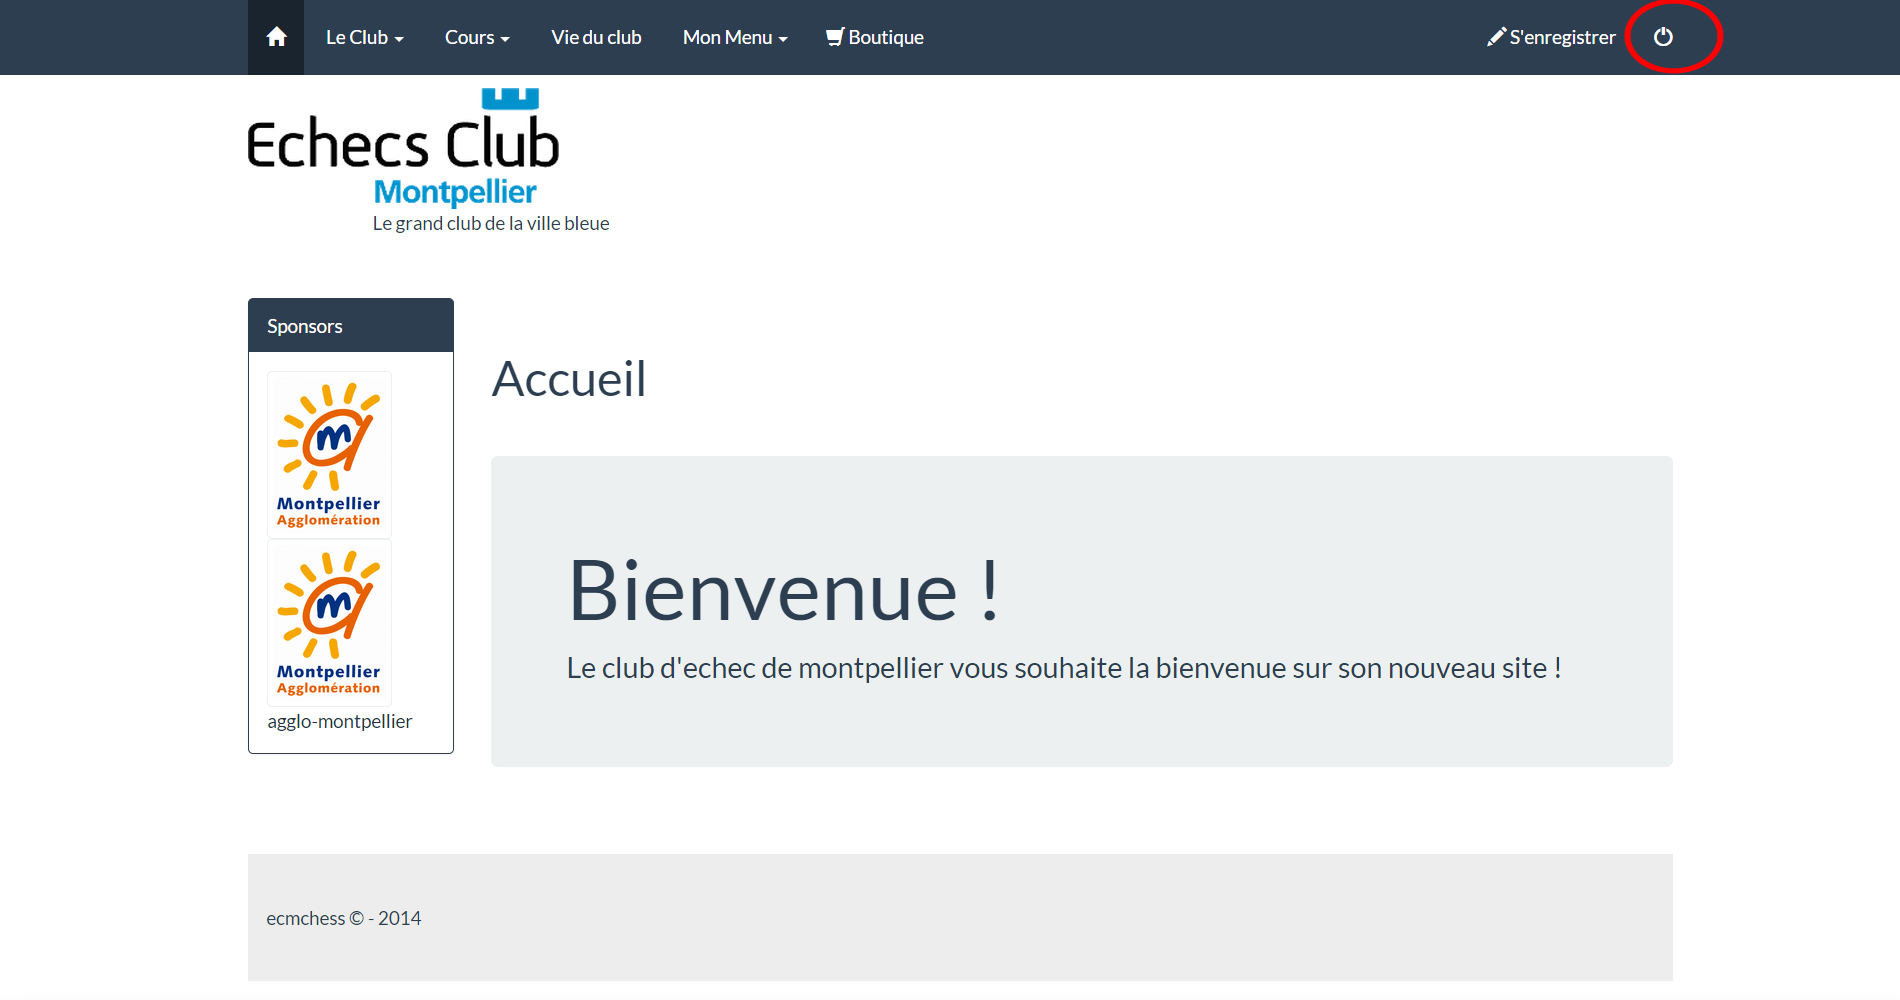
\includegraphics[scale=0.3]{images/acceuil-btn-connexion.png}
\end{figure}

\begin{figure} 
    \caption{Page de connexion}  
    \label{connexion}
    \centering
    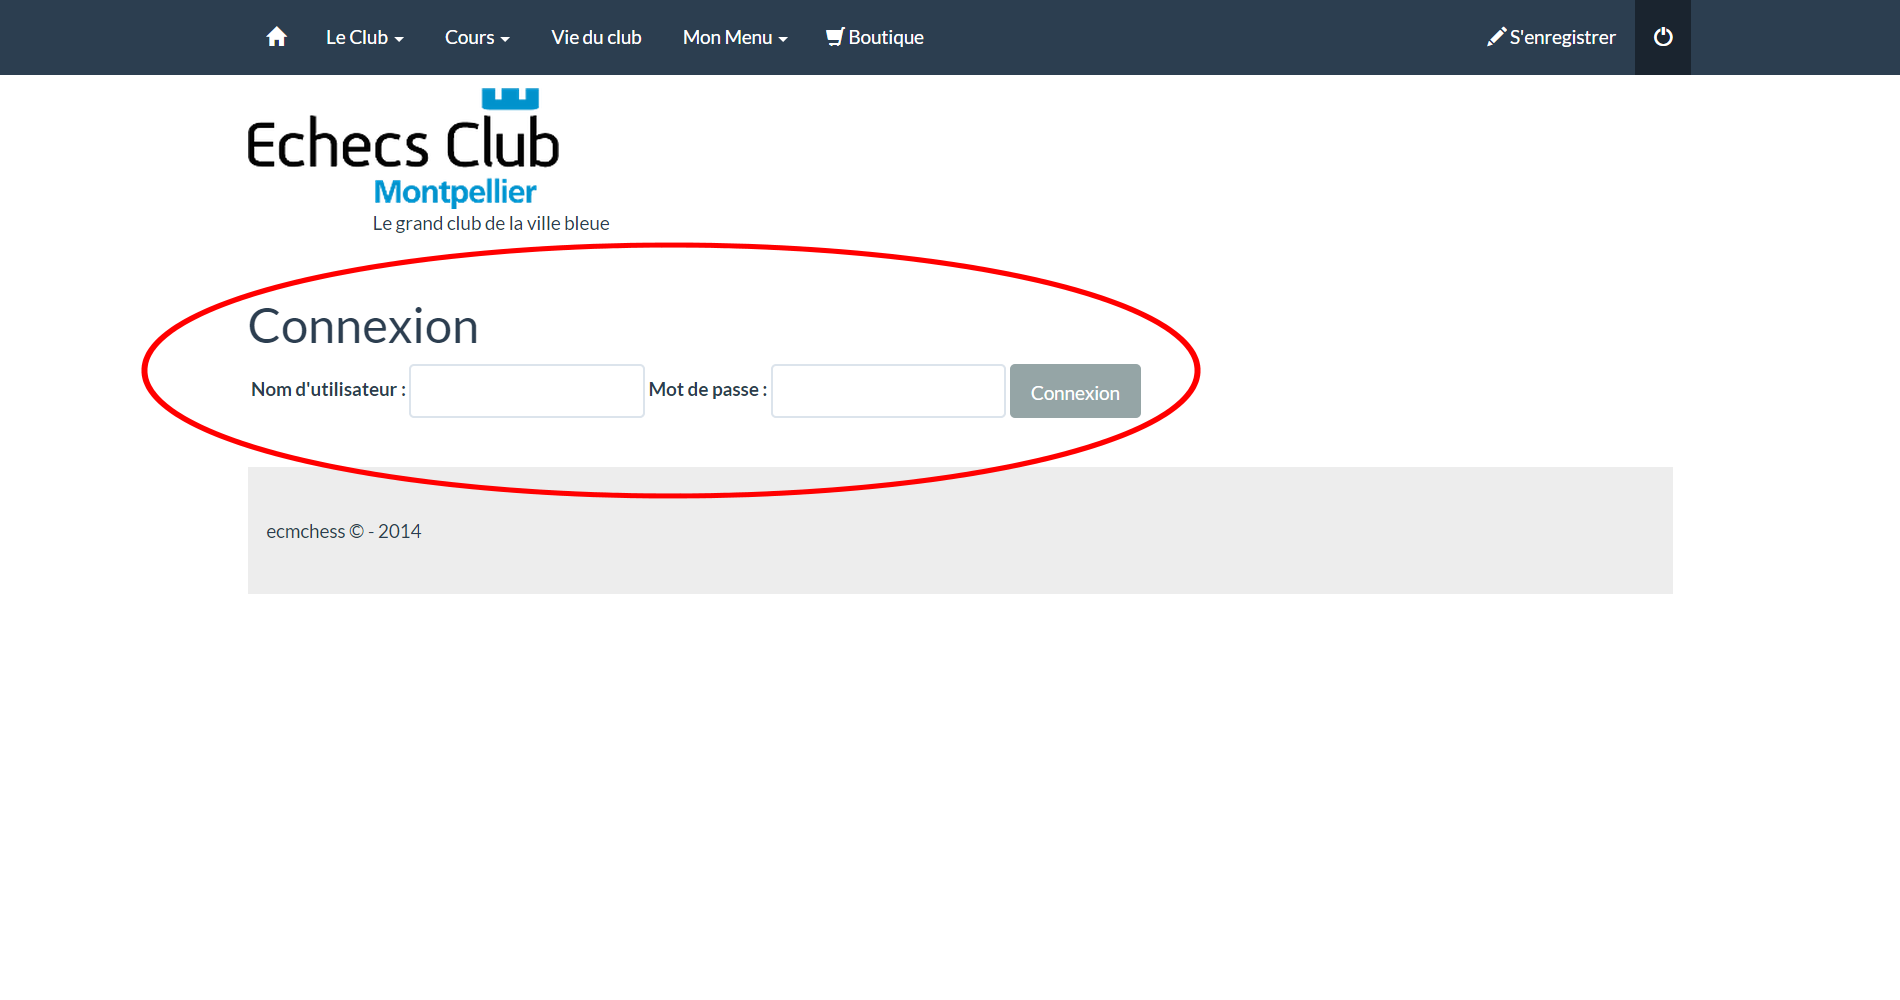
\includegraphics[scale=0.3]{images/connexion.png}
\end{figure}
Une fois connecté il faut cliquer sur le bouton Administration du menu (voir figure \ref{accueil-btn-admin}).
\begin{figure} 
    \caption{Bouton administration sur la page d'accueil}  
    \label{accueil-btn-admin}
    \centering
    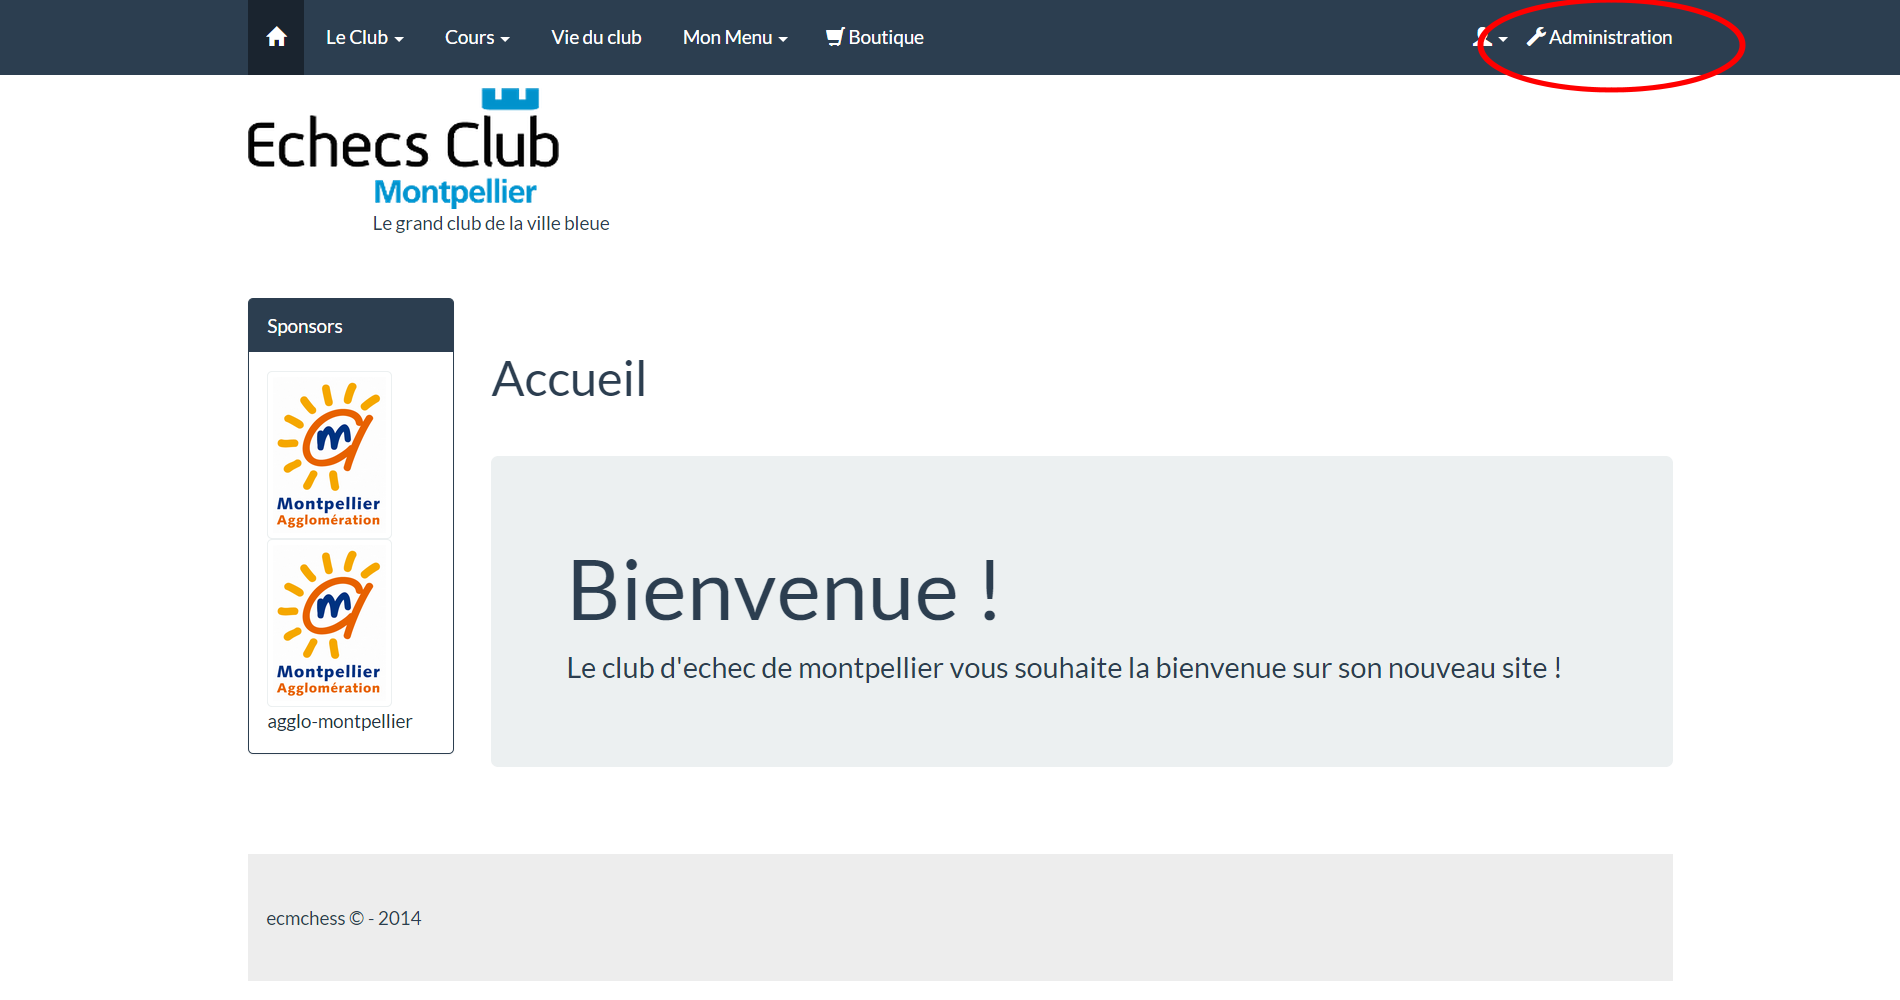
\includegraphics[scale=0.3]{images/btn-admin.png}
\end{figure}
Ensuite le site redirige automatiquement vers le back office (voir figure \ref{backoffice}).

\begin{figure} 
    \caption{Dashboard du back office}  
    \label{backoffice}
    \centering
    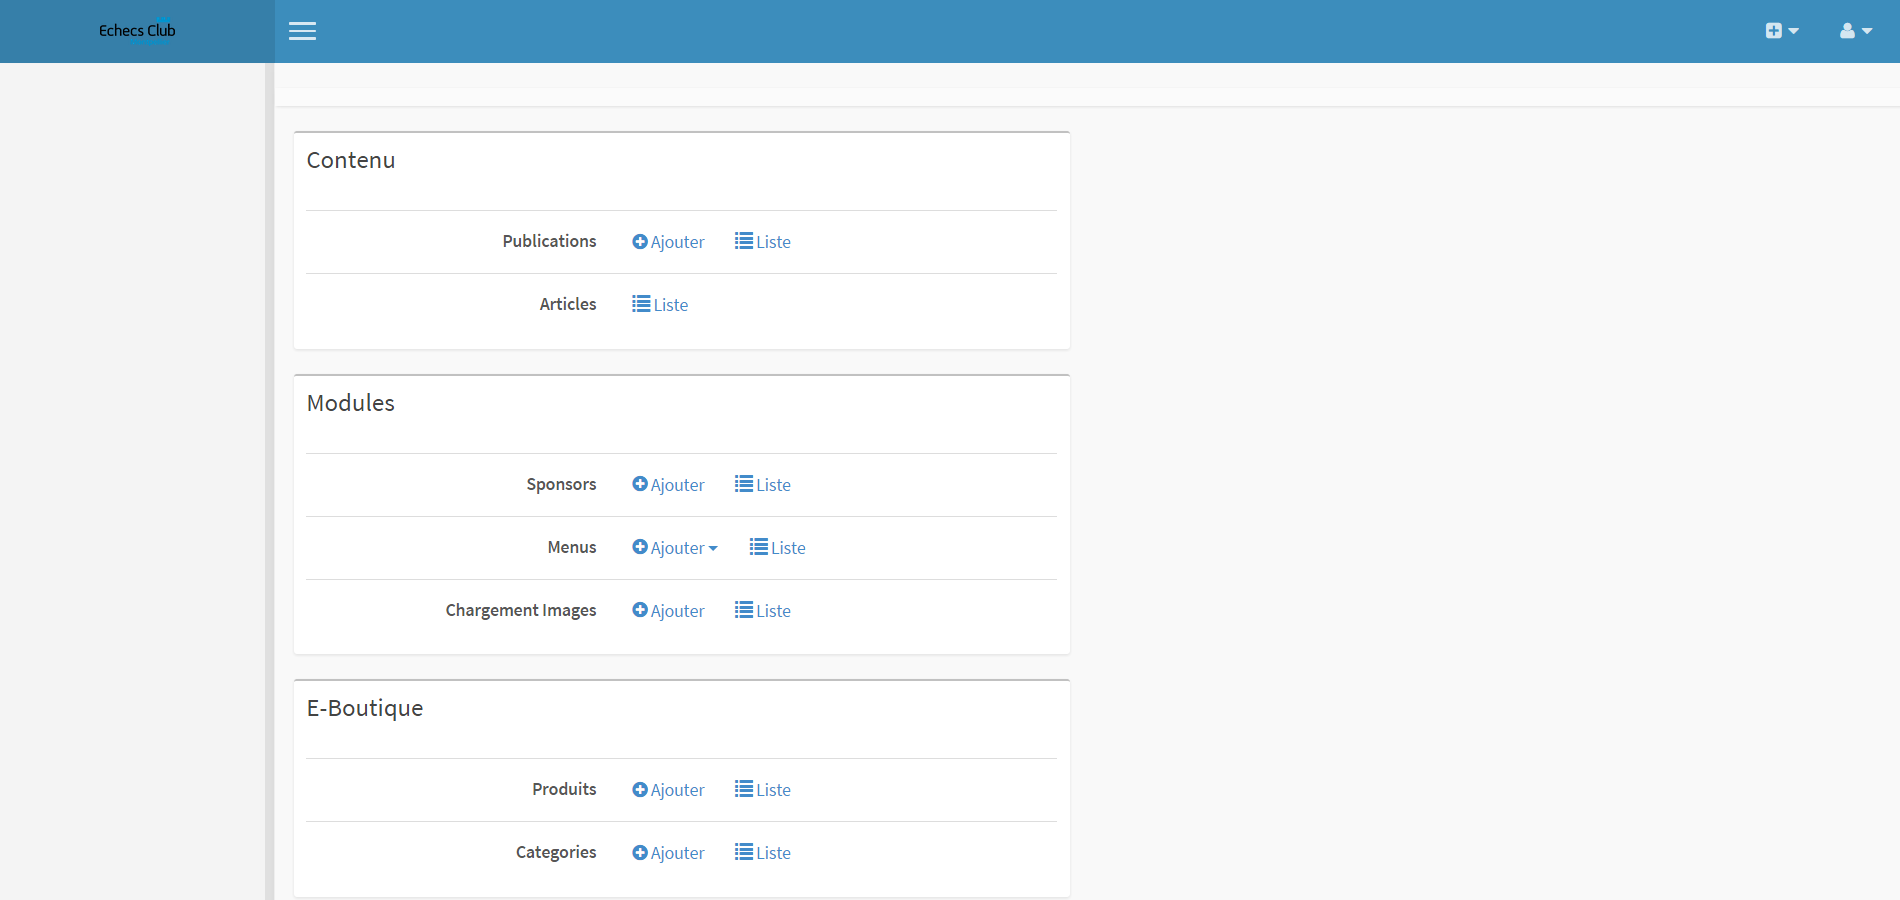
\includegraphics[scale=0.3]{images/backoffice.png}
\end{figure}
Le back office est constitué de trois blocs, le premier bloc “contenu” va servir à ajouter/modifier/supprimer une publication et à la modération des articles postés par les utilisateurs.

Ensuite le second bloc, intitulé “modules” sert à ajouter/modifier/supprimer/ordonner les sponsors, les menus,  les sous menu ,et a l’envoi d’images sur le serveur.

Pour finir, le dernier bloc sert à la gestion de la boutique, c’est dire à ajouter/modifier/supprimer des produits et des catégories.

Le fonctionnement du back office est sensiblement identique pour chaque item du site.
Tous ces items à l’exception des Articles ont un bouton “ajouter” qui permet d'être redirigé vers le formulaire d’ajout correspondant à l’item.
Il est aussi possible d’avoir la liste de toutes les entités par item.
Par exemple :  le bouton liste de la catégorie publication affichera la liste de toutes les publications qui sont enregistrées sur le site.
La page liste permet de modifier et de supprimer une entité de l’item sélectionné
La modification se déroule via le même formulaire que l’ajout, à la différence que, les champs sont pré-remplis avec les valeur de l’entité modifiée.

Pour illustrer le fonctionnement du back office, l’administration d’une publication et des sponsors vont être détaillés.
\chapter{Administration des publications}
Lors du clique sur le bouton liste le système affiche une page avec toutes les publications du site, chaque publication est modifiable et supprimable  via les boutons prévu à cet effet.
Il est possible aussi de modifier un article en cliquant sur son titre (voir figure \ref{liste-publication}).
\begin{figure} 
    \caption{Bouton connexion sur la page d'accueil}  
    \label{liste-publication}
    \centering
    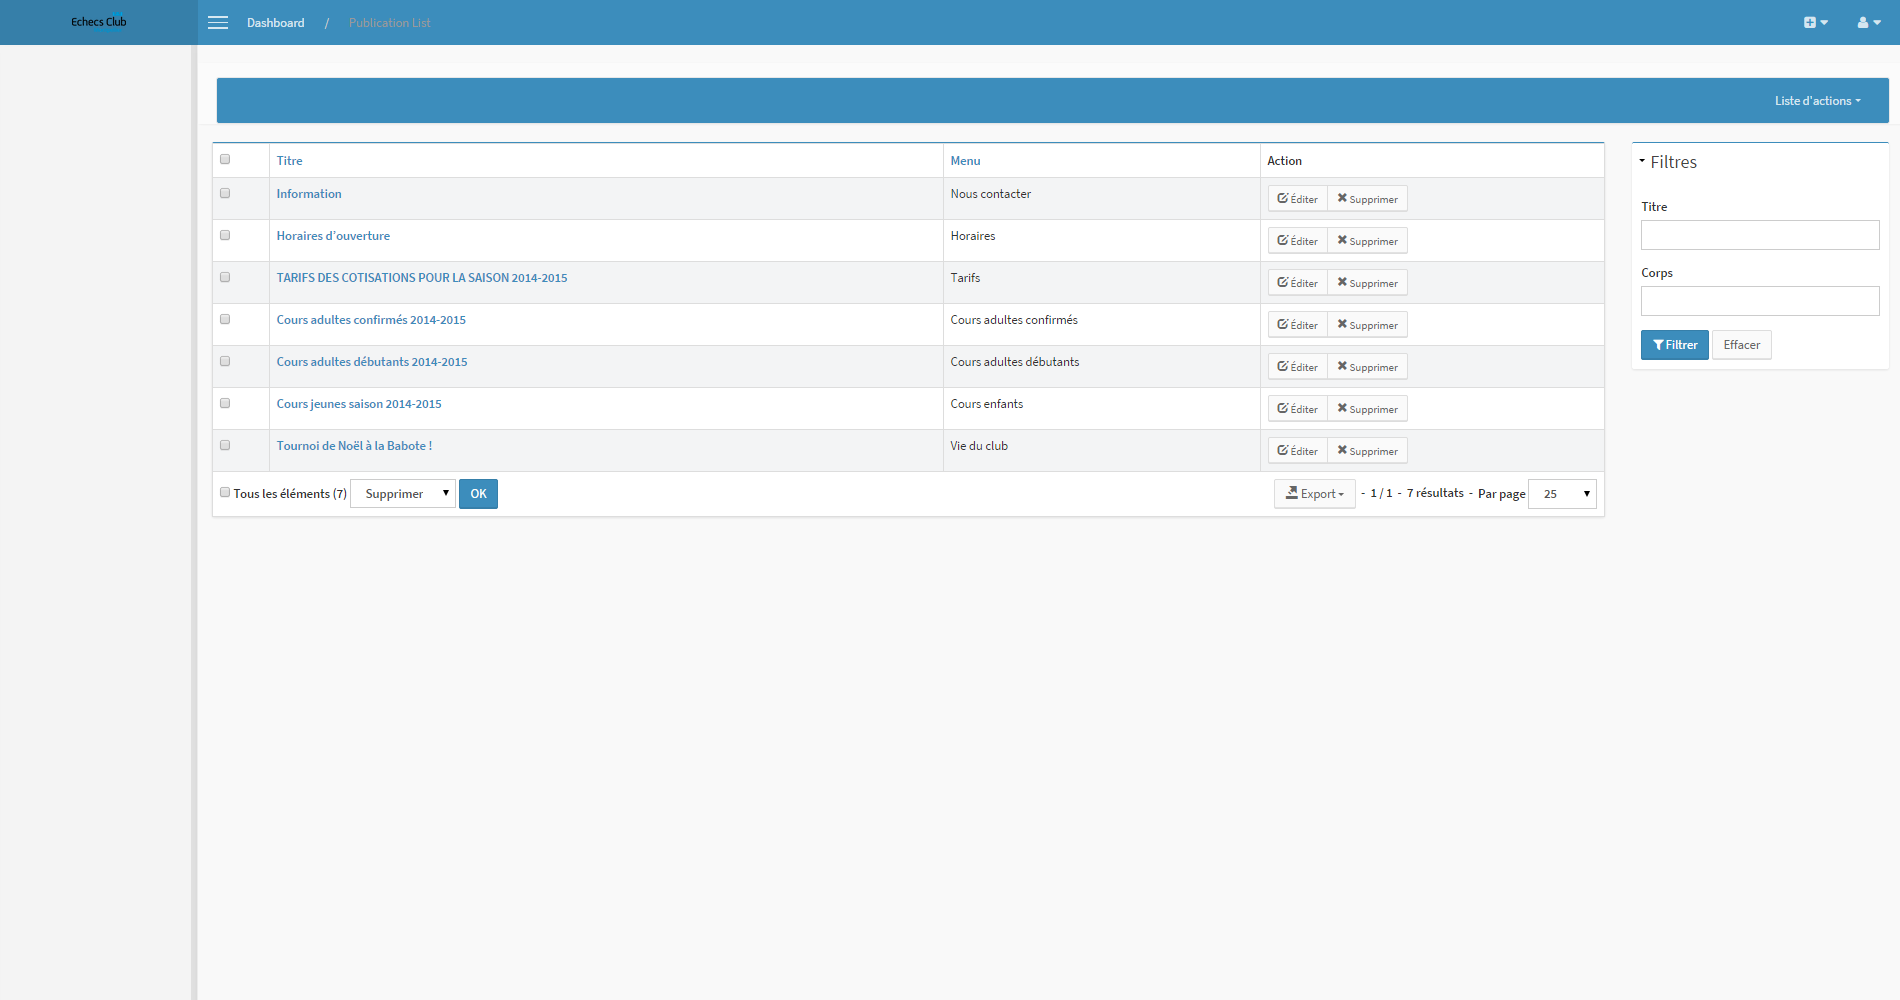
\includegraphics[scale=0.3]{images/liste-publication.png}
\end{figure}
Lorsque l’on souhaite modifier un article , le système nous redirige vers la page de modification.
Sur cette page il est possible de modifier le titre via la zone de texte correspondante,
le corps du texte, quand a lui se gère via un champ CKEditor (dont nous avons détaillé le fonctionnement précédemment ).
Il est aussi possible de modifier le menu dans lequel la publication sera affichée,
la liste déroulante correspondante contient les menus du site. 

Pour valider on peut soit cliquer sur “Mettre à  jour“ pour valider et rester sur la même page, soit cliquer sur  “Mettre à jour et fermer” ce qui enregistre les modification et renvoie sur la liste des publications. 

Le bouton supprimer sert, quant à lui, à supprimer la publication (voir figure \ref{modif-publication}).
\begin{figure} 
    \caption{Édition d'une publication}  
    \label{modif-publication}
    \centering
    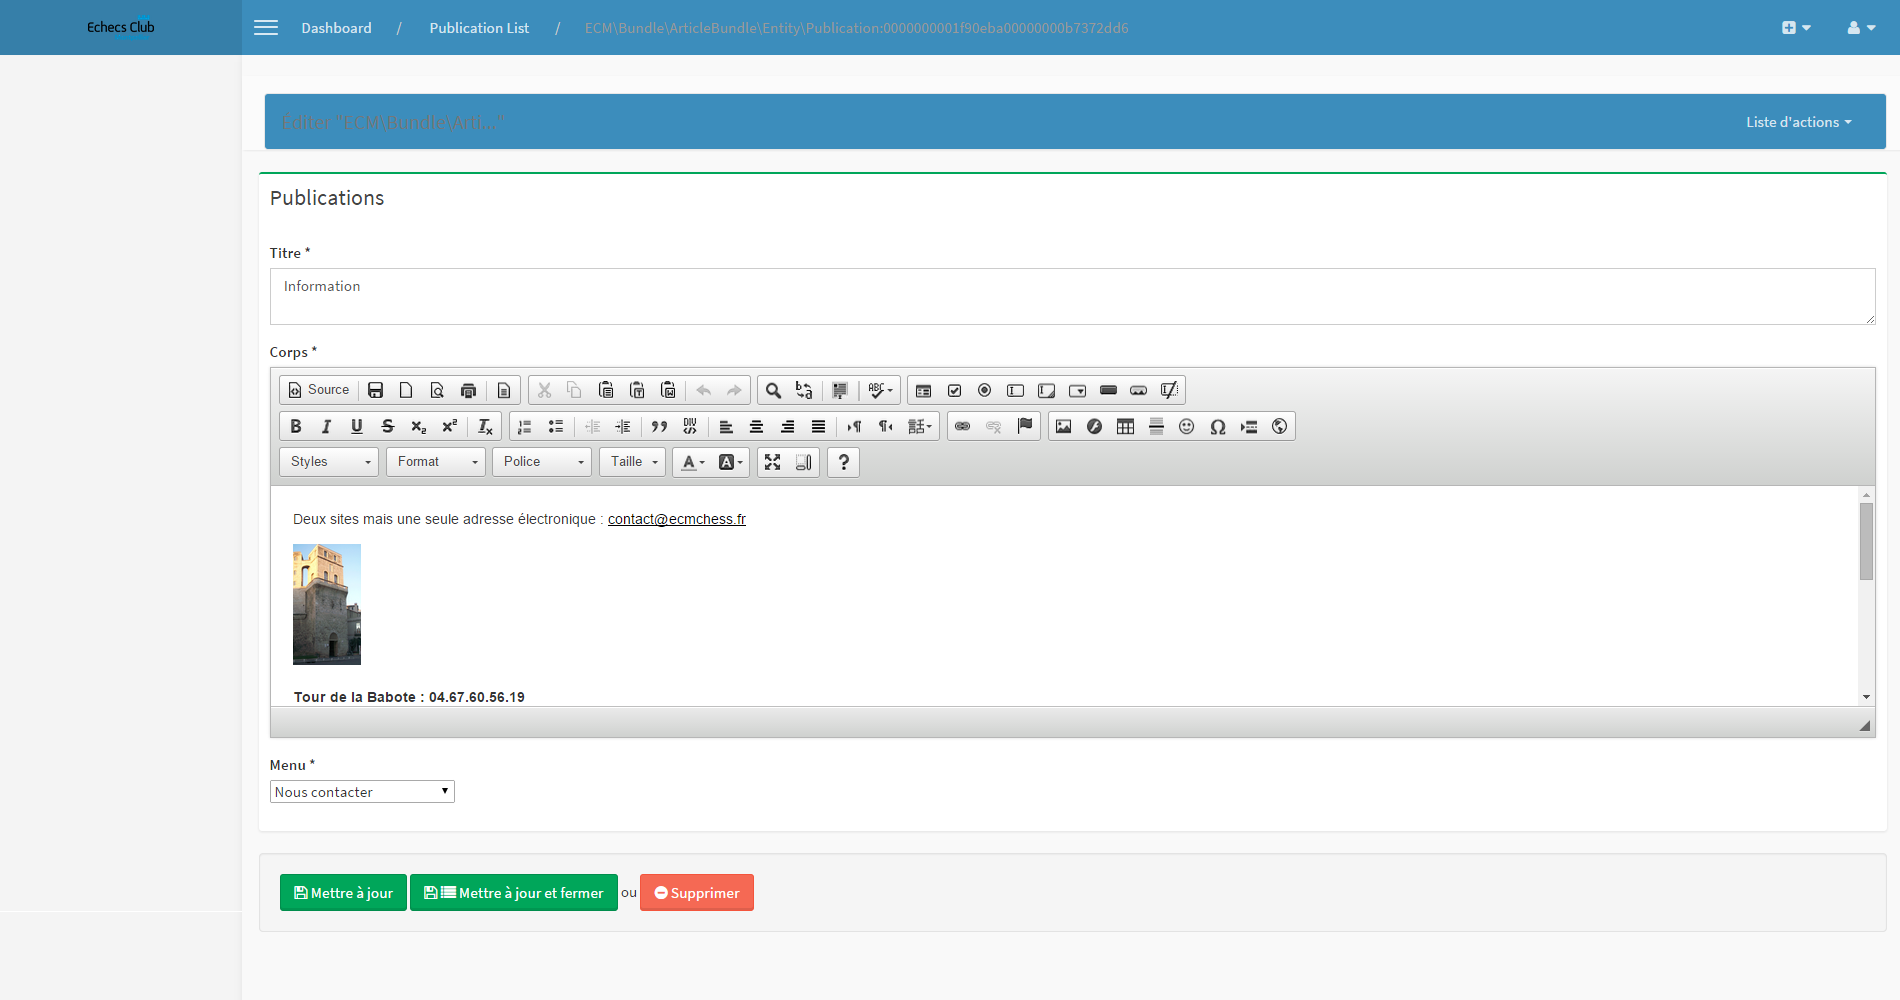
\includegraphics[scale=0.3]{images/modif-publication.png}
\end{figure}
Il est aussi possible d’ajouter une publication via le bouton “Ajouter”, sur la page d’accueil du back office, l’ajout d’une publication se fait via le formulaire suivant, dont le fonctionnement ne diffère pas de la modification (voir figure \ref{ajout-publication}).
\begin{figure} 
    \caption{Création d'une publication}  
    \label{ajout-publication}
    \centering
    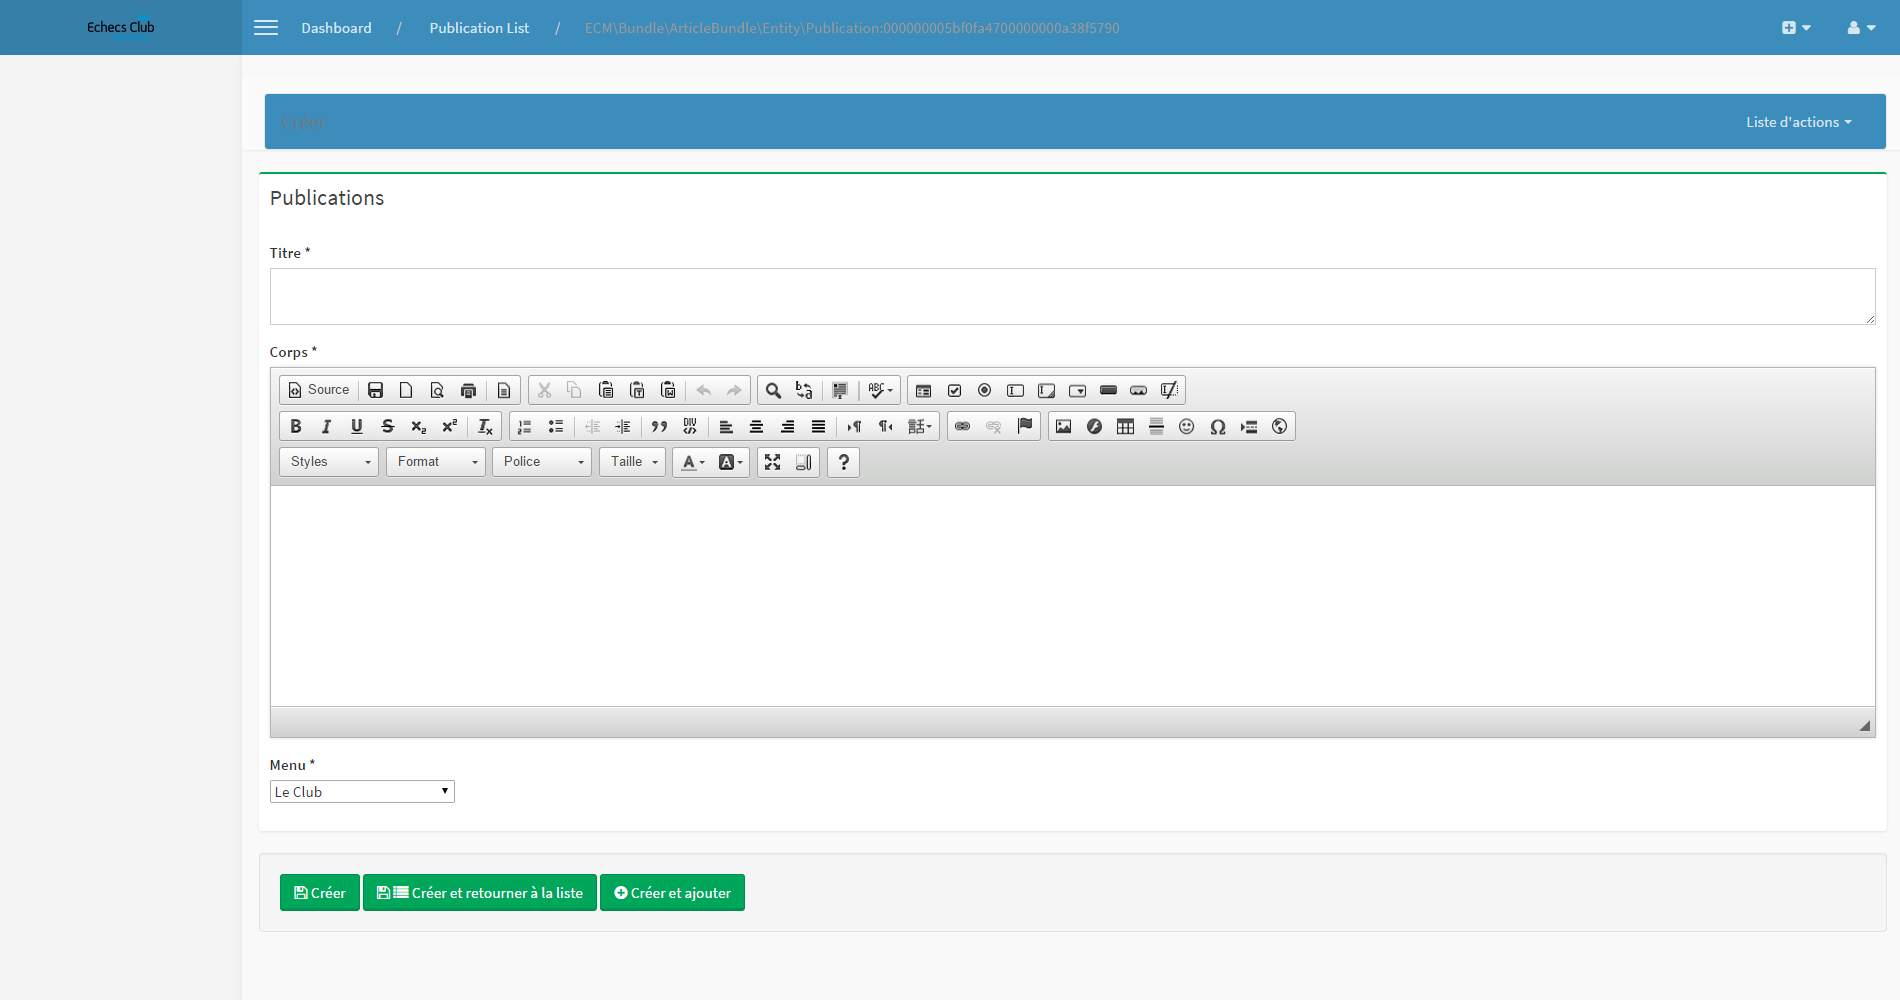
\includegraphics[scale=0.3]{images/ajout-publication.png}
\end{figure}

\chapter{Administration des sponsors}
Pour ajouter un sponsor il faut cliquer sur le bouton “ajouter” de la page d’accueil du back office dans la partie sponsor du bloc “module”, le système nous affiche alors le formulaire adéquat.

Il suffit alors de renseigner le titre, le lien vers lequel pointera le sponsor, l’image qui s’affichera (l’image n’est pas obligatoire) ainsi que sa position (voir figure \ref{ajout-sponsor}).
\begin{figure} 
    \caption{Création d'un sponsor}  
    \label{ajout-sponsor}
    \centering
    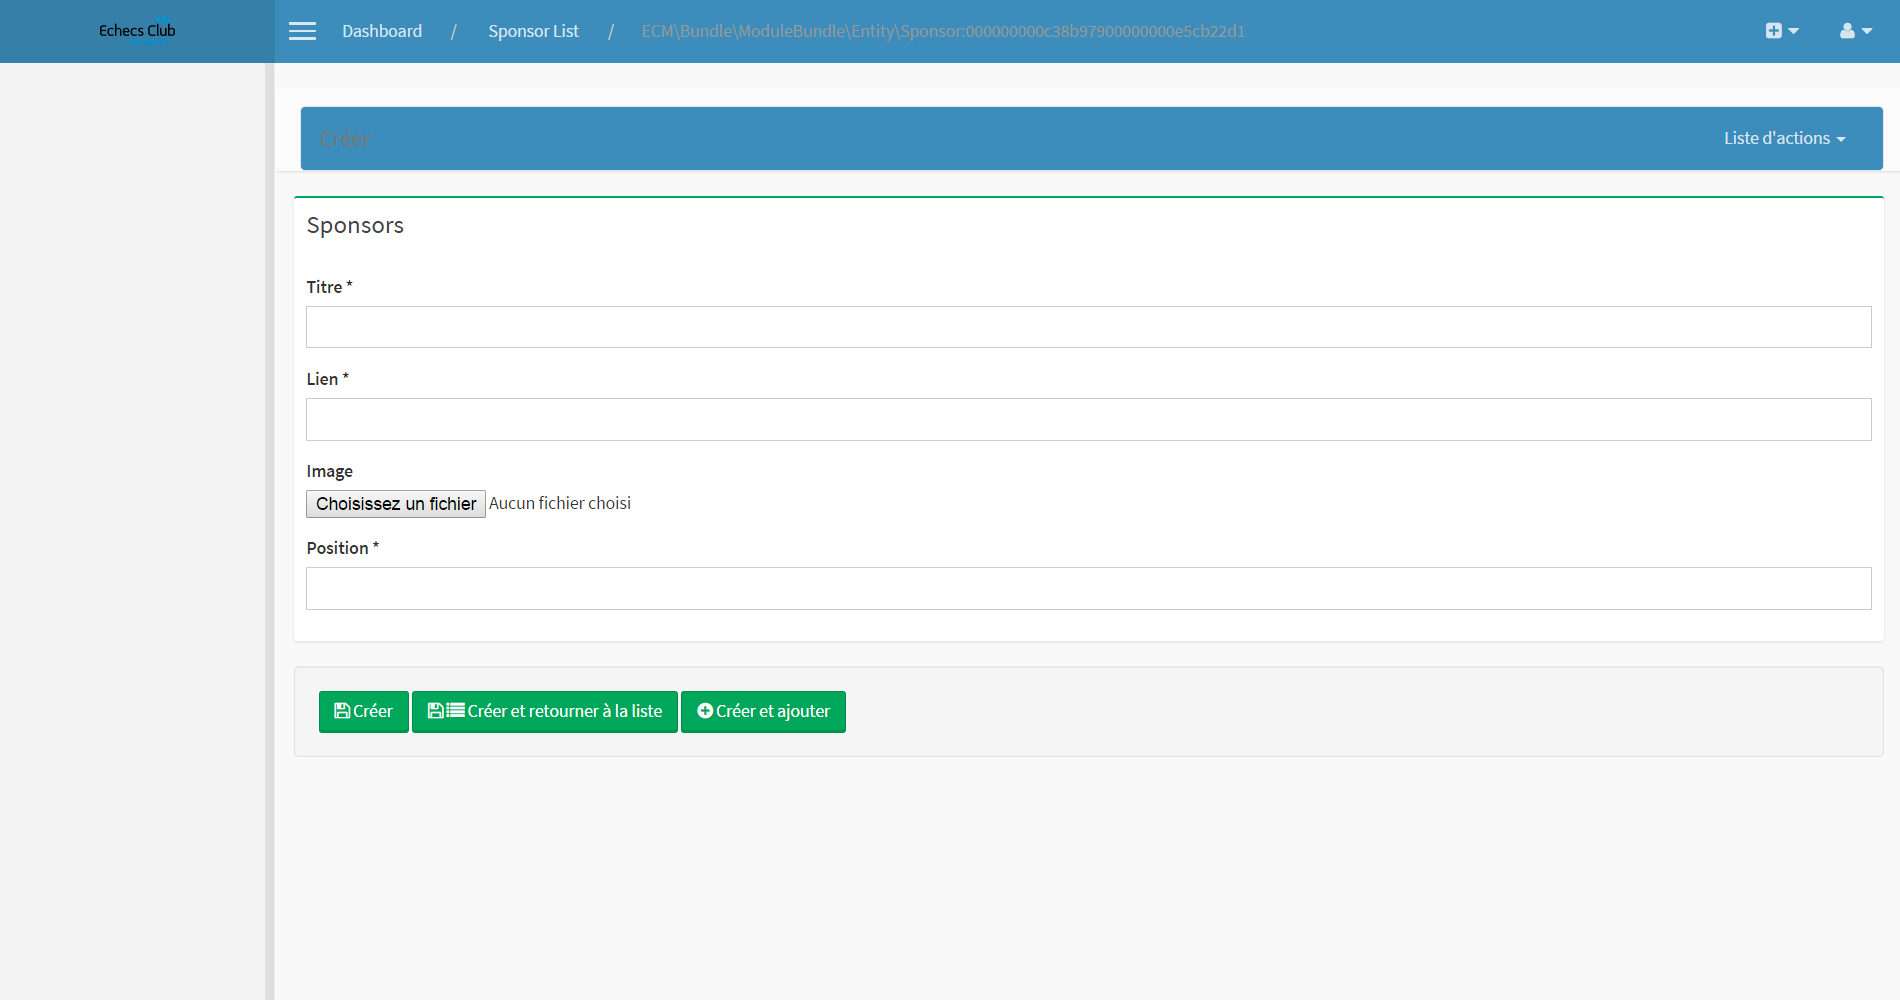
\includegraphics[scale=0.3]{images/ajoutSponsor.png}
\end{figure}
La modification se fait via un formulaire sensiblement identique. 

Il est aussi possible de modifier la position d’un sponsor de façon dynamique sur la page liste des sponsors, il suffit de cliquer sur les flèches pour faire monter ou descendre les sponsors (voir figure \ref{liste-sponsor}).
\begin{figure} 
    \caption{Liste des publications}  
    \label{liste-sponsor}
    \centering
    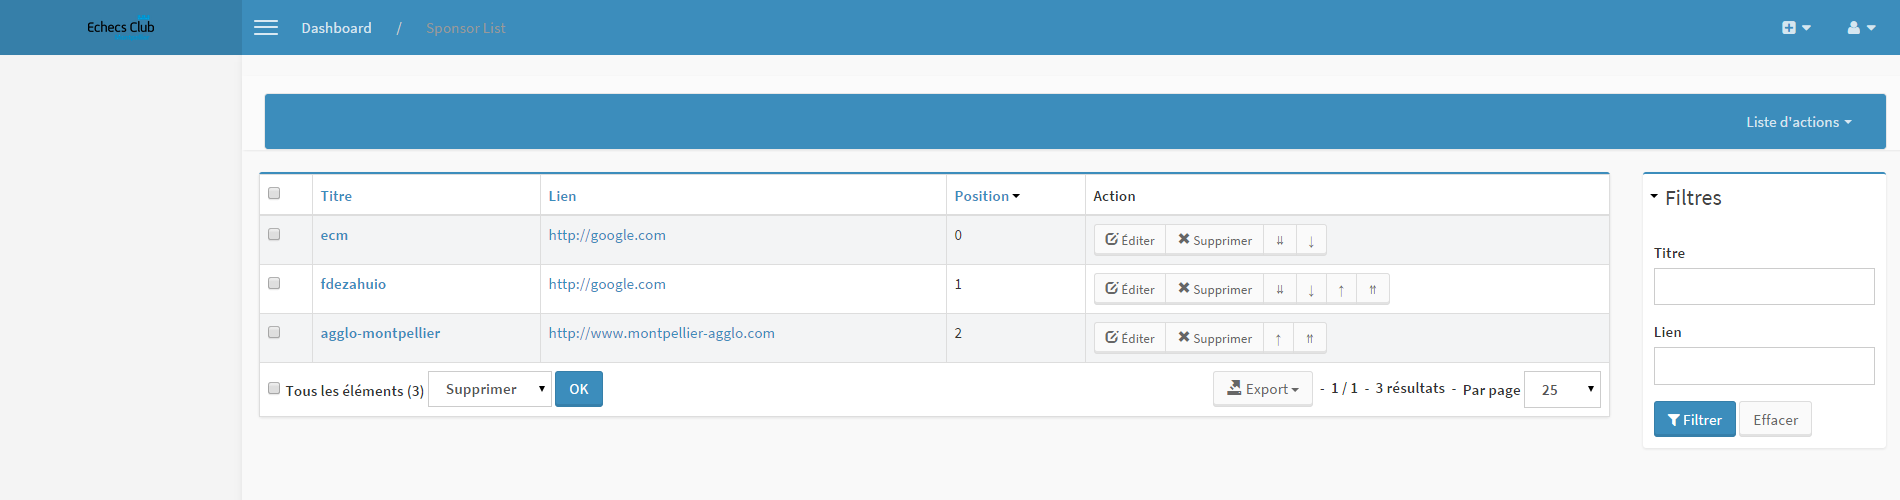
\includegraphics[scale=0.3]{images/liste-sponsor.png}
\end{figure}

\chapter*{Conclusion}
Nous avons réalisé le projet demandé en grande partie mais beaucoup d’améliorations et d’évolutions restent possibles, en effet, le site a fait peau neuve, possède une interface d’administration simple d’utilisation pour gérer l’architecture et le contenu du site, et permet à ses membres de poster (avec vérification préalable) des articles. Une vitrine permetant de présenter les produits a elle aussi été mise en place. En revanche, un panier pourrait être envisagé pour permettre aux utilisateur de faire leur commande en ligne. 
Cependant, certaines fonctionnalités n’ont pas pu être réalisées comme par exemple la gestion des équipes et une gestion plus approfondie des inscriptions.

Dans l’ensemble ce projet nous à permis de mieux appréhender les mécaniques de fonctionnement de Symphony, et nous a appris à nous méfier de l’installation hâtive de modules. Le travail en équipe nous a aussi poussé à utiliser des outils de travail communautaires (Git, Trello) qui sont largement utilisés en entreprise pour la gestion de projet.



% POST-TEXTES %
\appendix{}
\chapter{Script SQL phpmyadmin}
\lstinputlisting[language=sql]{localhost.sql}

\chapter{Diagramme des classes}
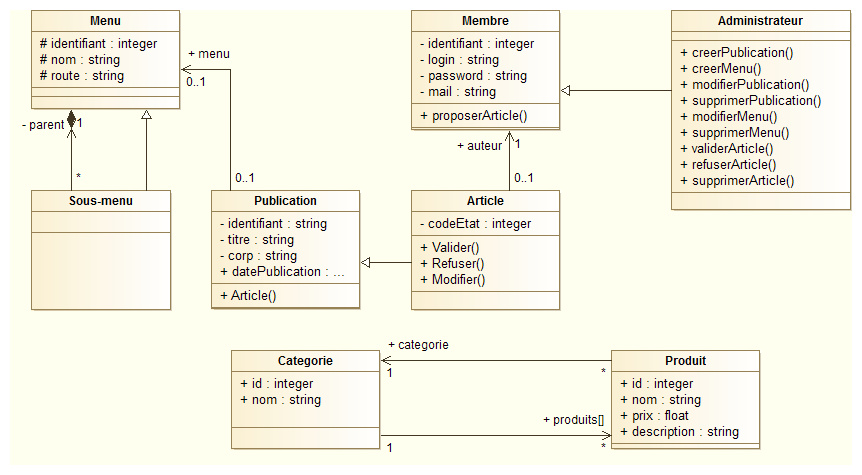
\includegraphics[scale=0.52]{images/diagramme-de-classe.png}

\listoffigures

\newpage
\pagestyle{empty}
\begin{abstract}
Le Projet ECMCHESS consiste à réaliser un site web vitrine pour un club d’échec montpellierain.
Ce dernier devait pouvoir fournir divers informations sur le club, informer ses membres et permettre l’achat de matériel d’échec via une boutique en ligne
Le site a été développé en utilisant le framework Symfony 2 ainsi que des modules notamment Bootstrap et Sonata.
mots-clés : Échecs, Club d’échec, Symfony 2, boutique en ligne.
\end{abstract}
\selectlanguage{english}
\begin{abstract}
ECMCHESS project consists in developping a website for a chessclub of Montpellier.
It was aimed to show various inforation about the club, display news and events to the club’s members and allow customer to buy chess’s stuff on an online store.
This web site has been developped using the Symfony 2 framework and bundles for instance Bootstrap and Sonata.

key words : Chess, chess club, symfony 2, e-shop.
\end{abstract}

\end{document}
